% Options for packages loaded elsewhere
\PassOptionsToPackage{unicode}{hyperref}
\PassOptionsToPackage{hyphens}{url}
%
\documentclass[
  oneside]{book}
\usepackage{amsmath,amssymb}
\usepackage{lmodern}
\usepackage{iftex}
\ifPDFTeX
  \usepackage[T1]{fontenc}
  \usepackage[utf8]{inputenc}
  \usepackage{textcomp} % provide euro and other symbols
\else % if luatex or xetex
  \usepackage{unicode-math}
  \defaultfontfeatures{Scale=MatchLowercase}
  \defaultfontfeatures[\rmfamily]{Ligatures=TeX,Scale=1}
\fi
% Use upquote if available, for straight quotes in verbatim environments
\IfFileExists{upquote.sty}{\usepackage{upquote}}{}
\IfFileExists{microtype.sty}{% use microtype if available
  \usepackage[]{microtype}
  \UseMicrotypeSet[protrusion]{basicmath} % disable protrusion for tt fonts
}{}
\makeatletter
\@ifundefined{KOMAClassName}{% if non-KOMA class
  \IfFileExists{parskip.sty}{%
    \usepackage{parskip}
  }{% else
    \setlength{\parindent}{0pt}
    \setlength{\parskip}{6pt plus 2pt minus 1pt}}
}{% if KOMA class
  \KOMAoptions{parskip=half}}
\makeatother
\usepackage{xcolor}
\IfFileExists{xurl.sty}{\usepackage{xurl}}{} % add URL line breaks if available
\IfFileExists{bookmark.sty}{\usepackage{bookmark}}{\usepackage{hyperref}}
\hypersetup{
  pdftitle={Booklet for the PiER},
  hidelinks,
  pdfcreator={LaTeX via pandoc}}
\urlstyle{same} % disable monospaced font for URLs
\usepackage{longtable,booktabs,array}
\usepackage{calc} % for calculating minipage widths
% Correct order of tables after \paragraph or \subparagraph
\usepackage{etoolbox}
\makeatletter
\patchcmd\longtable{\par}{\if@noskipsec\mbox{}\fi\par}{}{}
\makeatother
% Allow footnotes in longtable head/foot
\IfFileExists{footnotehyper.sty}{\usepackage{footnotehyper}}{\usepackage{footnote}}
\makesavenoteenv{longtable}
\usepackage{graphicx}
\makeatletter
\def\maxwidth{\ifdim\Gin@nat@width>\linewidth\linewidth\else\Gin@nat@width\fi}
\def\maxheight{\ifdim\Gin@nat@height>\textheight\textheight\else\Gin@nat@height\fi}
\makeatother
% Scale images if necessary, so that they will not overflow the page
% margins by default, and it is still possible to overwrite the defaults
% using explicit options in \includegraphics[width, height, ...]{}
\setkeys{Gin}{width=\maxwidth,height=\maxheight,keepaspectratio}
% Set default figure placement to htbp
\makeatletter
\def\fps@figure{htbp}
\makeatother
\setlength{\emergencystretch}{3em} % prevent overfull lines
\providecommand{\tightlist}{%
  \setlength{\itemsep}{0pt}\setlength{\parskip}{0pt}}
\setcounter{secnumdepth}{5}
\ifLuaTeX
  \usepackage{selnolig}  % disable illegal ligatures
\fi

\title{Booklet for the PiER}
\author{}
\date{\vspace{-2.5em}}

\begin{document}
\maketitle

{
\setcounter{tocdepth}{2}
\tableofcontents
}
\hypertarget{index}{%
\chapter{Background}\label{index}}

\begin{figure}

{\centering \includegraphics[width=0.3\linewidth]{index_files/figure-latex/logo-1} 

}

\caption{The logo for the PiER. The above-water pillar structure in red (symbolising the infrastructure) and water waves in blue (by analogy the piano stave) collectively illustrate the web-based PiER facilities enabling ab initio and real-time genetic target prioritisation.}\label{fig:logo}
\end{figure}

\begin{quote}
\textbf{Motivation}
\end{quote}

The field of target discovery has been advanced by genetics-led target prioritisation approaches. Integrative prioritisation for early-stage genetic target discovery has proven cost-effective in promoting the translational use of disease genetic associations, which is increasingly recognised in reducing drug attrition rate in late-stage clinical trials.

\begin{quote}
\textbf{Design}
\end{quote}

Building on the verified Pi approach (see \href{https://www.ncbi.nlm.nih.gov/pubmed/31253980}{Nature Genetics 2019}), here I introduce web-based servers/facilities called \texttt{PiER}. The PiER is free and open to all users and there is no login requirement, allowing the users to perform ab initio and real-time target prioritisation harnessing human disease genetics, functional genomics and protein interactions.

By analogy to the \href{https://www.piano-keyboard-guide.com/grand-staff.html}{piano stave}, the PiER consists of five horizontal lines, with three lines representing the elementary facility (\texttt{eV2CG}, \texttt{eCG2PG} and \texttt{eCrosstalk}), each doing specific tasks on their own, and the rest two lines signifying the combinatory facility (\texttt{cTGene} and \texttt{cTCrosstalk}).

\begin{itemize}
\item
  \protect\hyperlink{ev2cg}{eV2CG}, linking variants to core genes; see \href{/app/examples/_tmp_RMD_eV2CG.html}{Example Output}
\item
  \protect\hyperlink{ecg2pg}{eCG2PG}, networking core genes to peripheral genes; see \href{/app/examples/_tmp_RMD_eCG2PG.html}{Example Output}
\item
  \protect\hyperlink{ecrosstalk}{eCrosstalk}, identifying the crosstalk between pathways; see \href{/app/examples/_tmp_RMD_eCrosstalk.html}{Example Output}
\item
  \protect\hyperlink{ctgene}{cTGene}, prioritising targets at the gene level; see \href{/app/examples/_tmp_RMD_cTGene.html}{Example Output}
\item
  \protect\hyperlink{ctcrosstalk}{cTCrosstalk}, prioritising targets at the crosstalk level; see \href{/app/examples/_tmp_RMD_cTCrosstalk.html}{Example Output}
\end{itemize}

\hypertarget{facilities}{%
\chapter{Facilities}\label{facilities}}

The elementary facility supports three specific tasks, including three online tools: (i) \texttt{eV2CG}, utilising functional genomics to link disease-associated variants (including those located at the non-coding genome) to core genes likely responsible for genetic associations; (ii) \texttt{eCG2PG}, using knowledge of protein interactions to `network' core genes with each other and with additional peripheral genes as well, producing a ranked list of core and peripheral genes; and (iii) \texttt{eCrosstalk}, exploiting the information of pathway-derived interactions to identify highly ranked genes that mediate the crosstalk between molecular pathways. By chaining together elementary tasks supported in the elementary facility, the combinatory facility enables the automation of genetics-led and network-based integrative prioritisation for genetic targets, both at the gene level (\texttt{cTGene}) and at the crosstalk level (\texttt{cTCrosstalk}). Notably, in addition to target crosstalk, the \texttt{cTCrosstalk} further supports target pathway prioritisation and crosstalk-based drug repurposing analysis (that is, repositioning approved drugs from original disease indications into new ones).

\begin{figure}

{\centering \includegraphics[width=1\linewidth]{index_files/figure-latex/design-1} 

}

\caption{Schematic illustration of two facilities supported in the PiER.}\label{fig:design}
\end{figure}

\hypertarget{compatibility}{%
\chapter{Compatibility}\label{compatibility}}

\begin{table}

\caption{\label{tab:unnamed-chunk-3}A summary of the PiER browser compatibility.}
\centering
\begin{tabular}[t]{l|c|c|c}
\hline
  & MacOS (Big Sur) & Windows (10) & Linux (Ubuntu)\\
\hline
Safari & 14.1.2 & N/A & N/A\\
\hline
Microsoft Edge & N/A & 85.0.564.67 & N/A\\
\hline
Google Chrome & 96.0.4664.110 & 90.0.4430.93 & 96.0.4664.110\\
\hline
Firefox & 95.0.2 & 95.0.2 & 95.0.2\\
\hline
\end{tabular}
\end{table}

\hypertarget{runtime}{%
\chapter{Runtime}\label{runtime}}

\begin{table}

\caption{\label{tab:unnamed-chunk-4}A summary of the runtime (on the server and client sides) per tool estimated using Google Chrome.}
\centering
\begin{tabular}[t]{c|c|c}
\hline
Facilities & Tools & Runtime (Server + Client)\\
\hline
Elementary & eV2CG & (67 + 82) seconds\\
\hline
Elementary & eCG2PG & (15 + 70) seconds\\
\hline
Elementary & eCrosstalk & (53 + 71) seconds\\
\hline
Combinatory & cTGene & (90 + 91) seconds\\
\hline
Combinatory & cTCrosstalk & (143 + 97) seconds\\
\hline
\end{tabular}
\end{table}

\hypertarget{frontpage}{%
\chapter{Frontpage}\label{frontpage}}

\begin{figure}

{\centering \includegraphics[width=1\linewidth]{index_files/figure-latex/app-front-1} 

}

\caption{The landing frontpage (visited using Google Chrome in MacBook Pro) of the PiER, featuring two facilities (`elementary` and `combinatory`). The elementary facility includes: (i) `eV2CG`, linking disease associated variants (particularly located at the non-coding genomic region) to core genes likely responsible for genetic associations, based on either promoter capture Hi-C (PCHi-C, that is, conformation evidence), quantitative trait locus (QTL) mapping (that is, genetic regulation of gene expression or protein abundance), or simply genomic proximity; (ii) `eCG2PG`, using knowledge of protein interactions to ‘network’ core genes with each other and with additional peripheral genes as well, producing a ranked list of core and peripheral genes; and (iii) `eCrosstalk`, exploiting the information of pathway-derived interactions to identify highly-ranked genes that mediate the crosstalk between molecular pathways. By chaining together elementary tasks supported in the elementary facility, the combinatory facility enables automation of genetics-led and network-based integrative prioritisation for genetic targets: (iv) at the gene level (`cTGene`); and (v) at the crosstalk level (`cTCrosstalk`). Also included is the tutorial-like booklet (in an HTML format) describing step-by-step instructions on how to use.}\label{fig:app-front}
\end{figure}

\hypertarget{development}{%
\chapter{Development}\label{development}}

The PiER was developed using a next-generation Perl web framework \href{https://www.mojolicious.org}{Mojolicious} that requires nearly zero-effort maintenance for interface updates. The PiER was also built using \href{https://getbootstrap.com}{Bootstrap} that supports the mobile-first and responsive webserver. The source codes are made available at \href{https://github.com/23verse/pier}{GitHub}.

\begin{figure}

{\centering 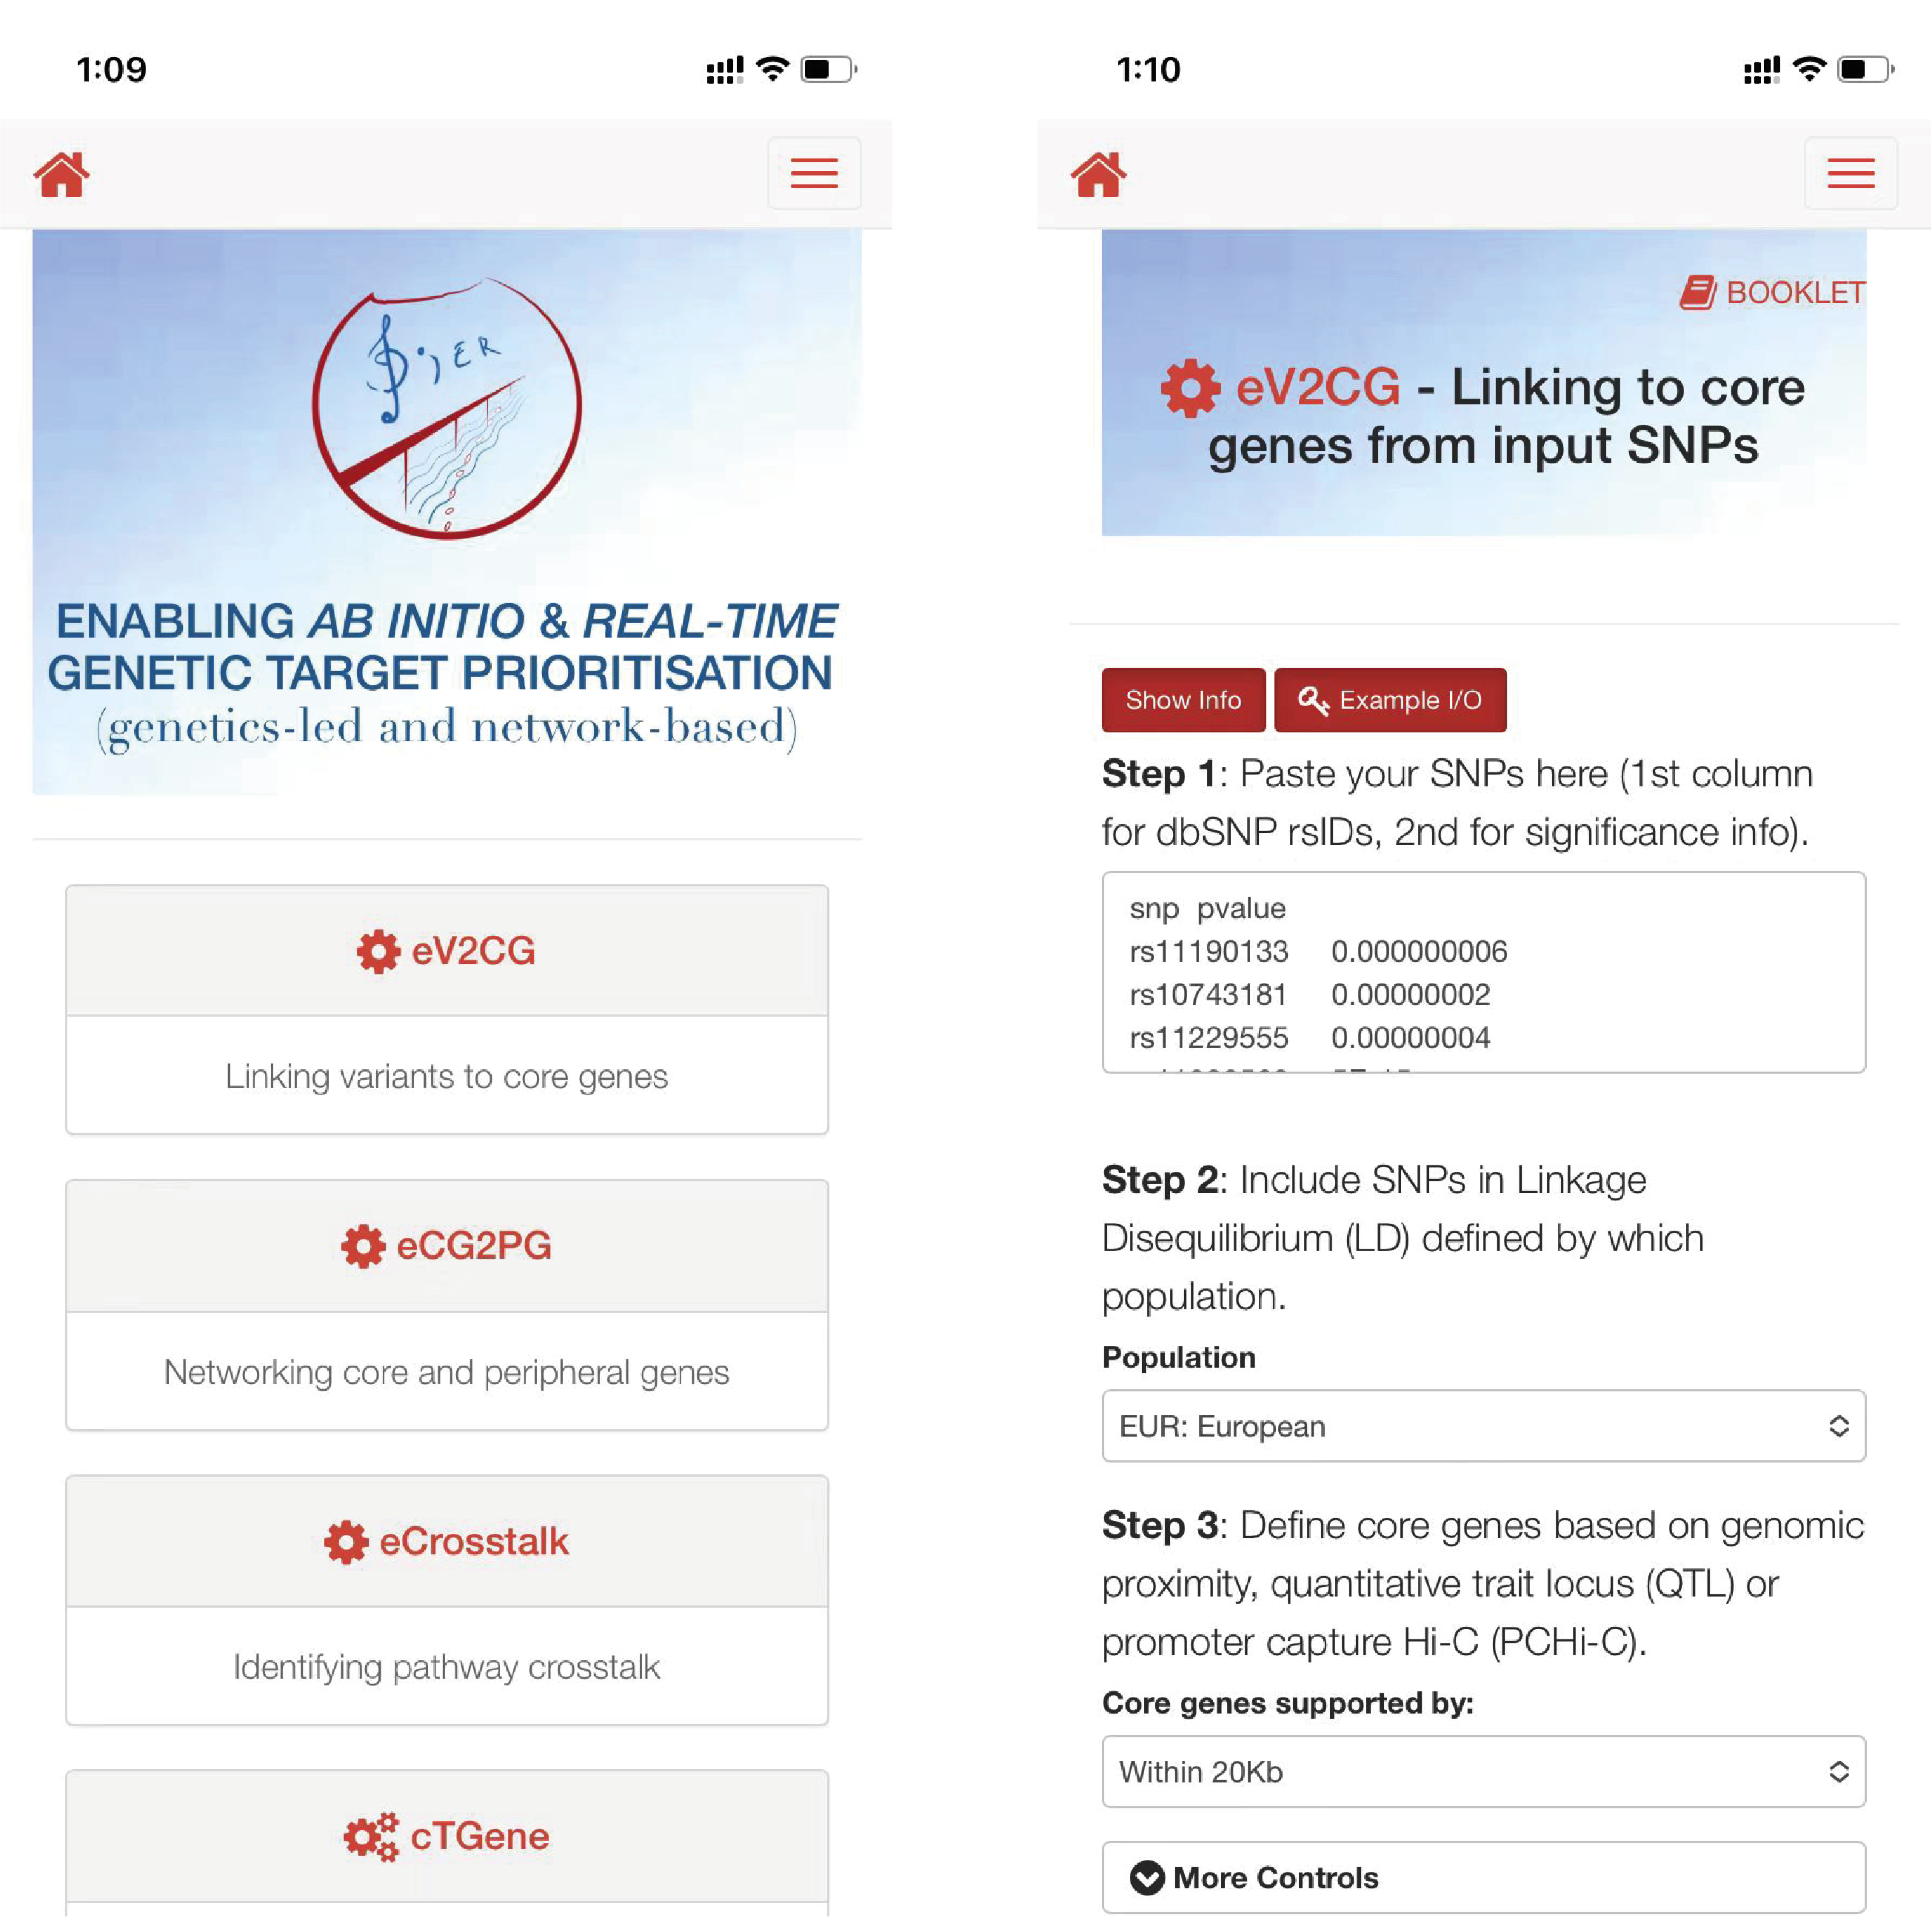
\includegraphics[width=0.7\linewidth]{index_files/figure-latex/app-iphone-1} 

}

\caption{The screenshots for the PiER visited using Google Chrome in iPhone. Left: the frontpage; Right: the `eV2CG` interface.}\label{fig:app-iphone}
\end{figure}

\hypertarget{help-buttons}{%
\chapter{Help buttons}\label{help-buttons}}

Each user-request interface has the \texttt{Show/Hide\ Info} toggle button that contains the help information on use, including the details on input, output, mechanism and other useful information, while the \texttt{Example\ I/O} button showcases the example input/output. For example, shown below is the screenshot in the \texttt{cTCrosstalk} interface.

\begin{figure}

{\centering 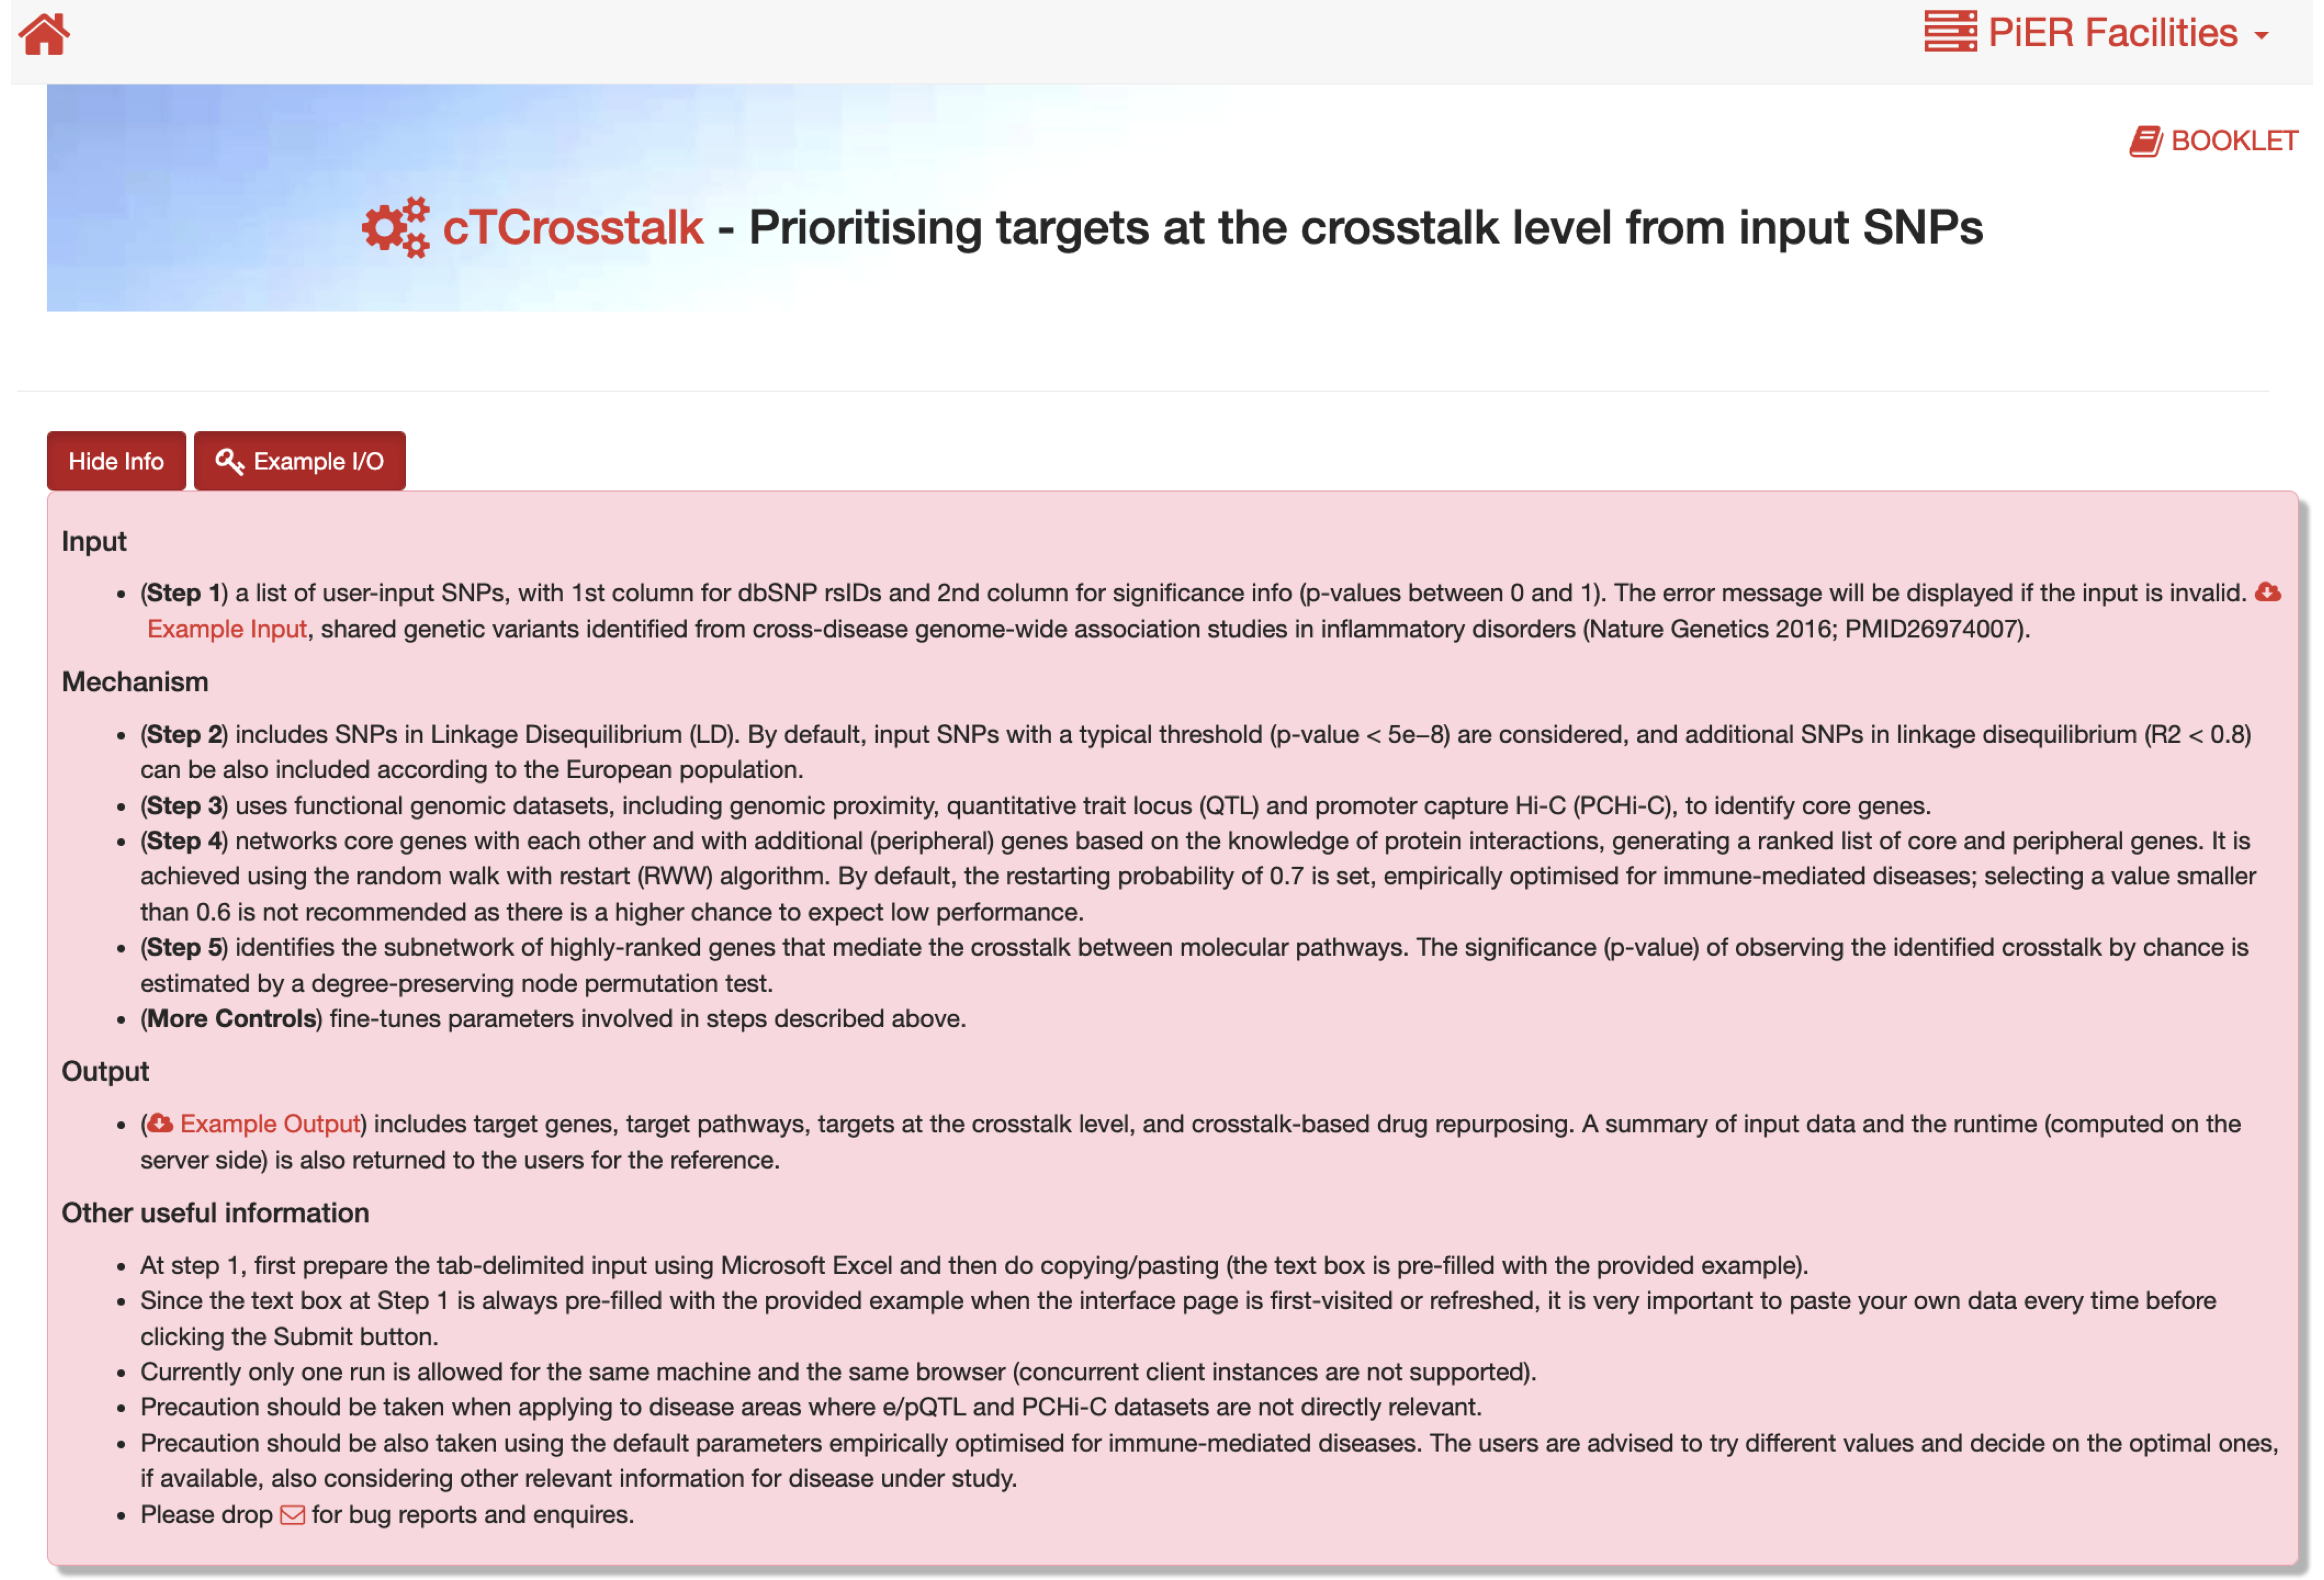
\includegraphics[width=1\linewidth]{index_files/figure-latex/cTCrosstalk-help-1} 

}

\caption{The screenshots for the `Show/Hide Info` toggle button in the `cTCrosstalk` interface.}\label{fig:cTCrosstalk-help}
\end{figure}

\hypertarget{error-messages}{%
\chapter{Error messages}\label{error-messages}}

The error messages will be displayed, for example, if the input into the \texttt{cTCrosstalk} is invalid (see the screenshot below). Notably, in the results page, a summary of input data is also returned to the users for the reference.

\begin{figure}

{\centering \includegraphics[width=1\linewidth]{index_files/figure-latex/cTCrosstalk-error-1} 

}

\caption{The screenshot for the error messages shown when the input is invalid, for example, in the `cTCrosstalk` interface.}\label{fig:cTCrosstalk-error}
\end{figure}

\hypertarget{ev2cg}{%
\chapter{eV2CG}\label{ev2cg}}

\hypertarget{interface}{%
\section{Interface}\label{interface}}

\begin{quote}
\textbf{Input}
\end{quote}

\begin{itemize}
\tightlist
\item
  \texttt{Step\ 1}: a list of user-input SNPs, with 1st column for dbSNP rsIDs and 2nd column for significance info (p-values between 0 and 1). The error message will be displayed if the input is invalid. Example input data are shared genetic variants identified from cross-disease genome-wide association studies in inflammatory disorders; see \href{https://www.ncbi.nlm.nih.gov/pubmed/26974007}{Nature Genetics 2016}.
\end{itemize}

\begin{quote}
\textbf{Mechanism}
\end{quote}

\begin{itemize}
\item
  \texttt{Step\ 2}: includes SNPs in Linkage Disequilibrium (LD). By default, input SNPs with a typical threshold (p-value \textless{} 5e−8) are considered, and additional SNPs in linkage disequilibrium (R2 \textless{} 0.8) can be also included according to the European population.
\item
  \texttt{Step\ 3}: uses genomic proximity, quantitative trait locus (QTL), or promoter capture Hi-C (PCHi-C) to identify core genes.
\item
  \texttt{More\ Controls}: fine-tunes parameters involved in steps described above.
\end{itemize}

\begin{quote}
\textbf{Output}
\end{quote}

\begin{itemize}
\tightlist
\item
  \href{/app/examples/_tmp_RMD_eV2CG.html}{Example Output} includes two interactive tables for core genes and evidence used, and a manhattan plot (illustrating scored core genes color-coded by chromosomes). A summary of input data and the runtime (computed on the server side) is also returned to the users for the reference.
\end{itemize}

\begin{figure}

{\centering \includegraphics[width=1\linewidth]{index_files/figure-latex/eV2CG-interface-1} 

}

\caption{The interface of eV2CG, linking disease associated variants (particularly located at the non-coding genomic region) to (core) genes likely responsible for associations, based on either promoter capture Hi-C (PCHi-C; conformation evidence), quantitative trait locus (QTL) mapping (that is, genetic regulation of gene expression or protein abundance), or simply genomic proximity. The `Show/Hide Info` toggle button contains the help information on how to use the `eV2CG`, including input, output, mechanism, etc.}\label{fig:eV2CG-interface}
\end{figure}

\hypertarget{linking-results}{%
\section{Linking results}\label{linking-results}}

\begin{itemize}
\item
  Under the tab \texttt{Output:\ core\ genes}, \texttt{Manhattan\ plot} illustrates scored core genes that are color-coded by chromosomes. Also provided is the downloadable PDF file.
\item
  Under the tab \texttt{Output:\ core\ genes}, \texttt{An\ interactive\ table} lists core genes linked from the input SNPs, with scores quantifying the level of genes responsible for genetic associations (capped at 100). Genes are cross-referenced and hyperlinked to GeneCards. Also provided is the column Evidence used to define core genes.
\item
  Under the tab \texttt{Output:\ core\ genes}, \texttt{Evidence\ table} for core genes, showing which SNPs (see the column \texttt{SNPs}) are used to define core genes (the column \texttt{Core\ genes}) based on which evidence (see the column \texttt{Evidence}). The column \texttt{SNP\ type} tells the SNP type (either \texttt{Input} for use-input SNPs or \texttt{LD} for LD SNPs). Notably, the column \texttt{Evidence} details datasets used: the prefix \texttt{Proximity\_} indicative of SNPs in the proximity, the prefix \texttt{PCHiC\_} for PCHi-C datasets, and the prefix \texttt{QTL\_} for e/pQTL datasets.
\end{itemize}

\begin{figure}

{\centering \includegraphics[width=0.8\linewidth]{index_files/figure-latex/eV2CG-results-1} 

}

\caption{Interactive results for the `eV2CG`. Under the tab `Output: core genes` is a manhattan plot illustrating scores for core genes. The user-input data under the tab `Input into eV2CG` are also returned for the exploration.}\label{fig:eV2CG-results}
\end{figure}

\begin{figure}

{\centering 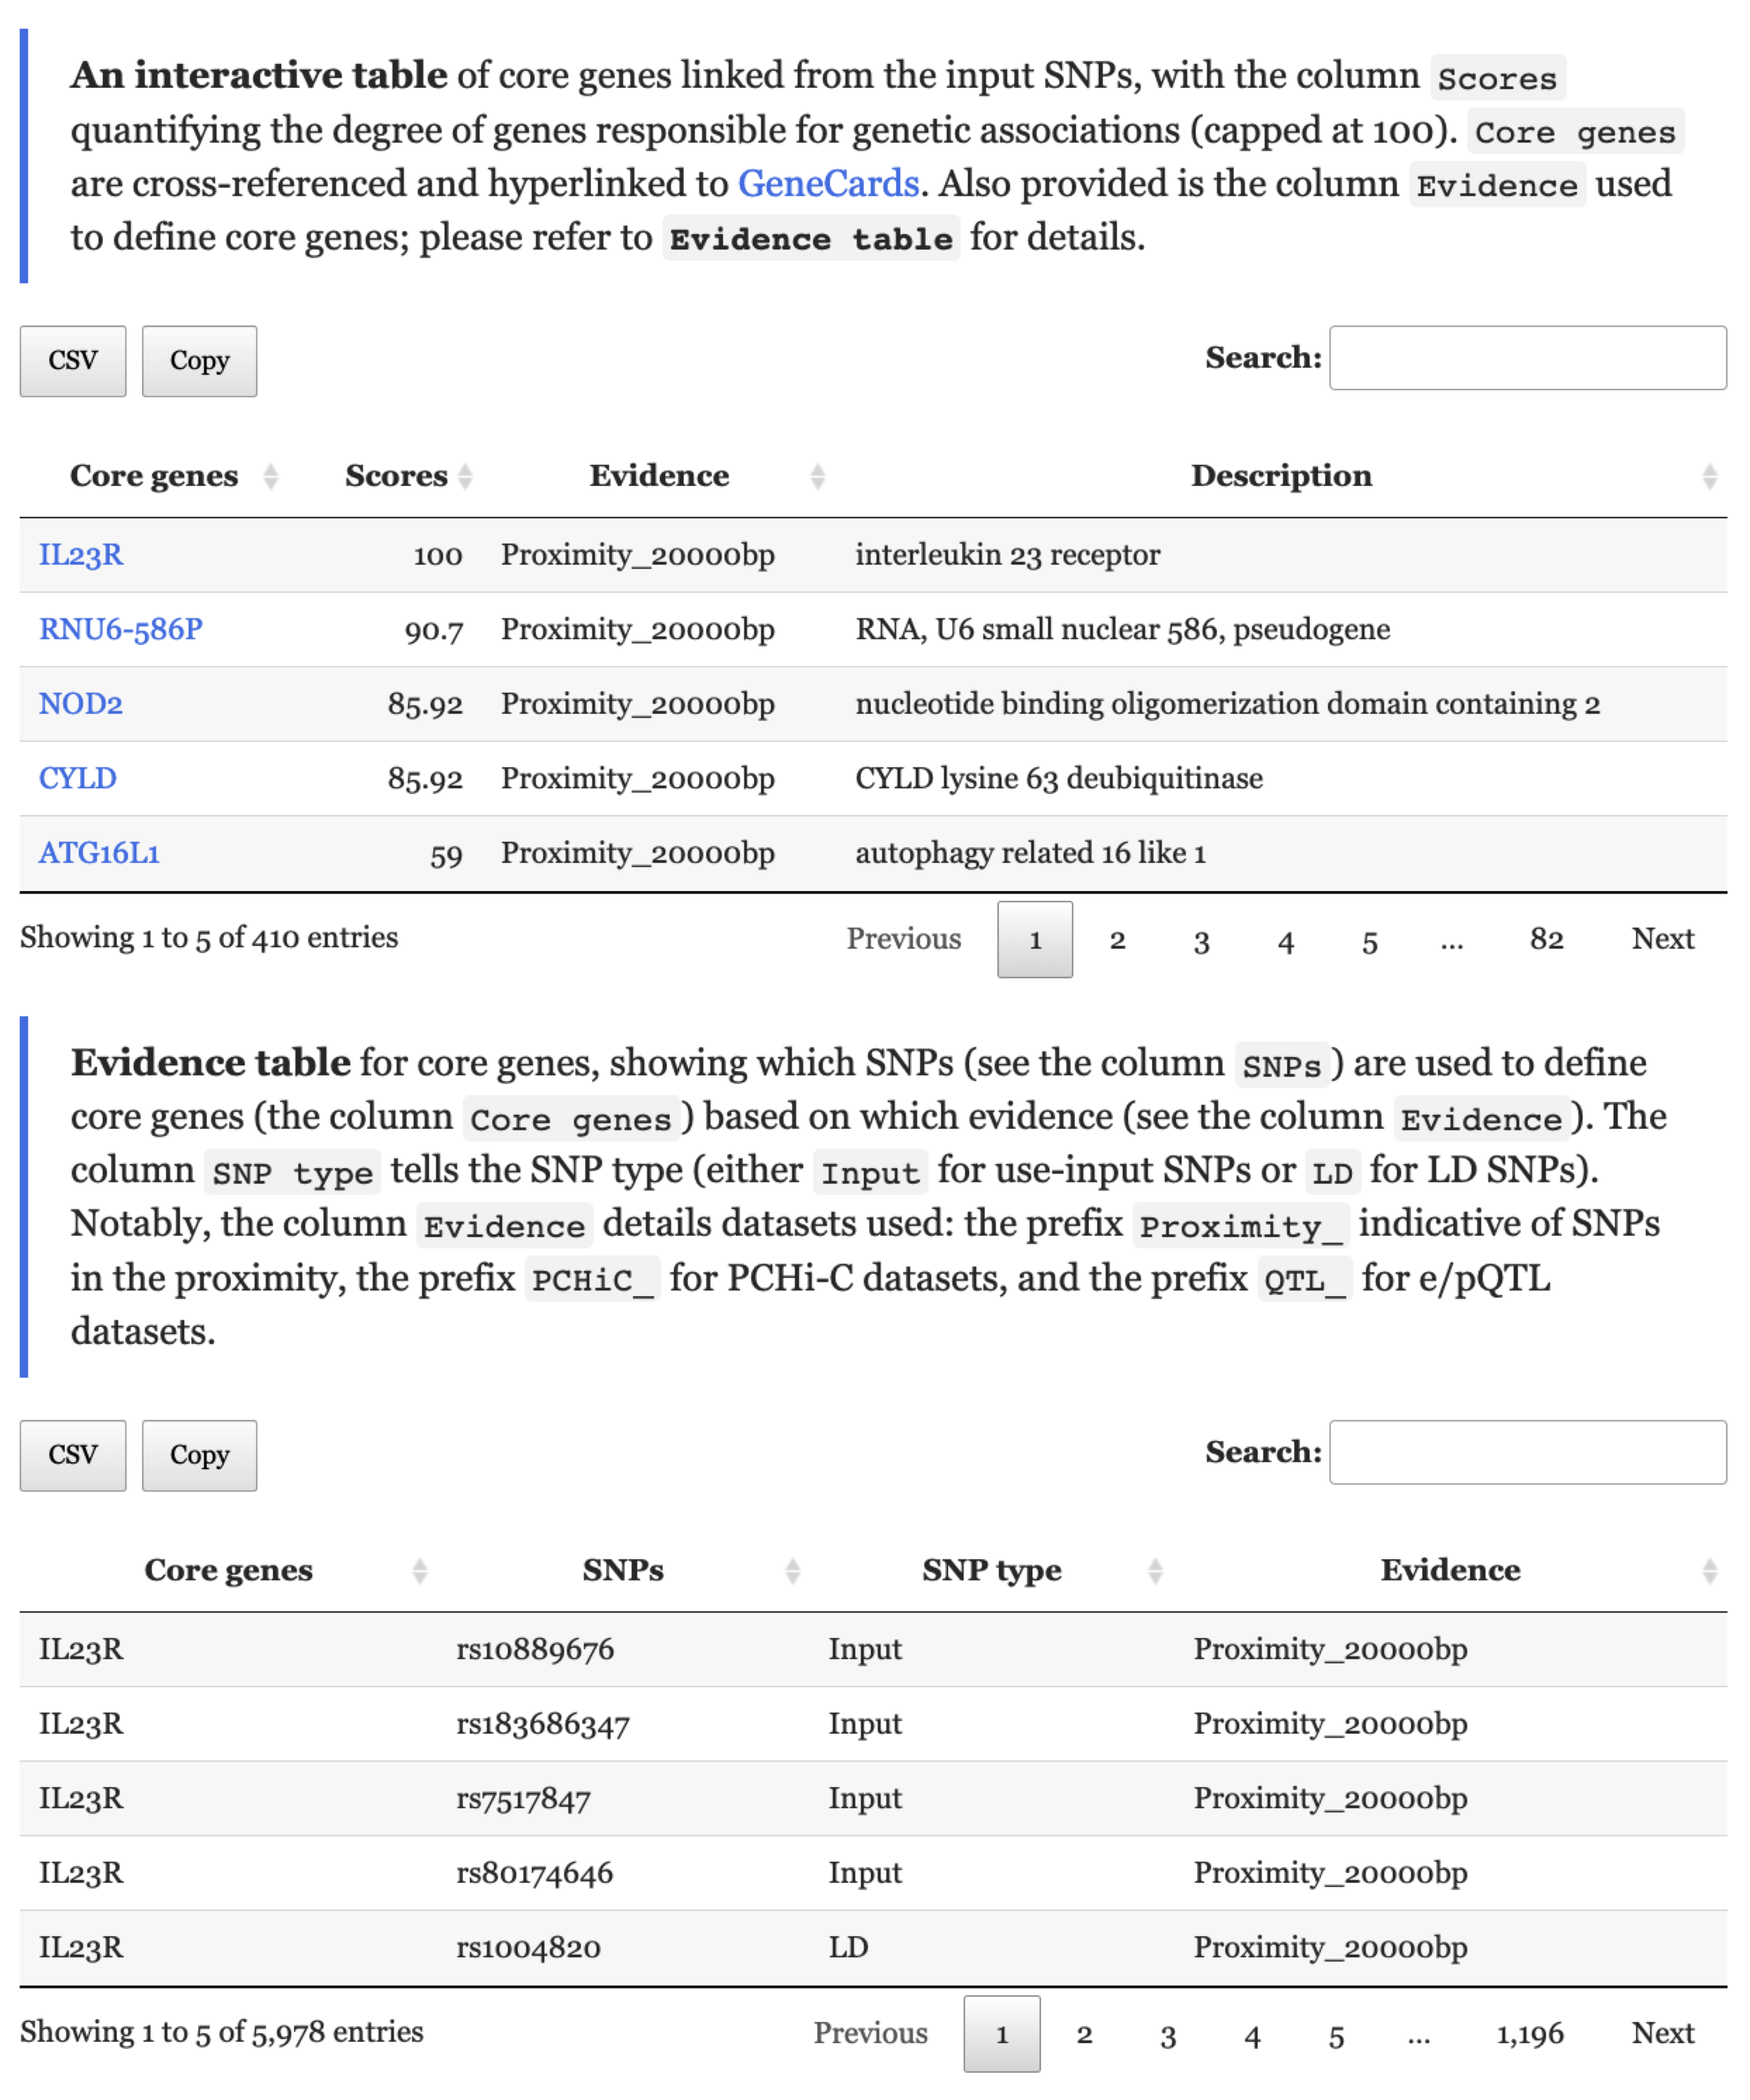
\includegraphics[width=0.9\linewidth]{index_files/figure-latex/eV2CG-evidence-1} 

}

\caption{Two tabular displays about core genes (top) and evidence (bottom) under the tab `Output: core genes`.}\label{fig:eV2CG-evidence}
\end{figure}

\hypertarget{ecg2pg}{%
\chapter{eCG2PG}\label{ecg2pg}}

\hypertarget{interface-1}{%
\section{Interface}\label{interface-1}}

\begin{quote}
\textbf{Input}
\end{quote}

\begin{itemize}
\tightlist
\item
  \texttt{Step\ 1}: a list of user-defined core genes, with 1st column for gene symbols, 2nd columns for weights (positive values), such as results from \texttt{eV2CG} above. The error message will be displayed if the input is invalid.
\end{itemize}

\begin{quote}
\textbf{Mechanism}
\end{quote}

\begin{itemize}
\item
  \texttt{Step\ 2}: networks core genes with each other and with additional (peripheral) genes based on the knowledge of protein interactions, generating a ranked list of core and peripheral genes. It is achieved using the random walk with restart (RWW) algorithm. By default, the restarting probability of 0.7 is set, empirically optimised for immune-mediated diseases; selecting a value smaller than 0.6 is not recommended as there is a higher chance to expect low performance.
\item
  \texttt{More\ Controls}: fine-tunes parameters involved in steps described above.
\end{itemize}

\begin{quote}
\textbf{Output}
\end{quote}

\begin{itemize}
\tightlist
\item
  \href{/app/examples/_tmp_RMD_eCG2PG.html}{Example Output} includes an interactive table for core and peripheral genes, and a manhattan plot (illustrating scores for genes color-coded by chromosomes). A summary of input data and the runtime (computed on the server side) is also returned to the users for the reference.
\end{itemize}

\begin{figure}

{\centering \includegraphics[width=1\linewidth]{index_files/figure-latex/eCG2PG-interface-1} 

}

\caption{The interface of the `eCG2PG`, using the knowledge of protein interactions to ‘network’ core genes with each other and with additional (peripheral) genes as well, generating a ranked list of core and peripheral genes. The `Show/Hide Info` toggle button contains the help information on how to use the `eCG2PG`, including input, output, mechanism, etc.}\label{fig:eCG2PG-interface}
\end{figure}

\hypertarget{networking-results}{%
\section{Networking results}\label{networking-results}}

\begin{itemize}
\item
  Under the tab \texttt{Output:\ core\ and\ peripheral\ genes}, \texttt{Manhattan\ plot} illustrates affinity scores for genes that are color-coded by chromosomes. Also provided is the downloadable PDF file.
\item
  Under the tab \texttt{Output:\ core\ and\ peripheral\ genes}, \texttt{An\ interactive\ table} lists core and peripheral genes, with scores quantifying the affinity to core genes (sum up to 1). Genes are cross-referenced and hyperlinked to GeneCards.
\end{itemize}

\begin{figure}

{\centering \includegraphics[width=0.8\linewidth]{index_files/figure-latex/eCG2PG-results-1} 

}

\caption{Interactive results for the `eCG2PG` under the tab `Output: core and peripheral genes`. The user-input data the tab `Input into eCG2PG` are also returned for the exploration.}\label{fig:eCG2PG-results}
\end{figure}

\hypertarget{ecrosstalk}{%
\chapter{eCrosstalk}\label{ecrosstalk}}

\hypertarget{interface-2}{%
\section{Interface}\label{interface-2}}

\begin{quote}
\textbf{Input}
\end{quote}

\begin{itemize}
\tightlist
\item
  \texttt{Step\ 1}: a ranked list of genes, with 1st column for gene symbols, 2nd columns for scores (positive values), such as results from \texttt{eCG2PG} above. The error message will be displayed if the input is invalid.
\end{itemize}

\begin{quote}
\textbf{Mechanism}
\end{quote}

\begin{itemize}
\tightlist
\item
  \texttt{Step\ 2}: identifies the subnetwork of highly-ranked genes that mediate the crosstalk between molecular pathways. The significance (p-value) of observing the identified crosstalk by chance is estimated by a degree-preserving node permutation test.
\end{itemize}

\begin{quote}
\textbf{Output}
\end{quote}

\begin{itemize}
\tightlist
\item
  \href{/app/examples/_tmp_RMD_eCrosstalk.html}{Example Output} includes an interactive table for pathway crosstalk genes, and a network visualisation (illustrating the crosstalk between pathways).
\end{itemize}

\begin{figure}

{\centering \includegraphics[width=1\linewidth]{index_files/figure-latex/eCrosstalk-interface-1} 

}

\caption{The interface of the `eCrosstalk`, exploiting the information of well-curated pathway-derived interactions to identify the subnetwork of highly ranked genes that mediate pathway crosstalk. The `Show/Hide Info` toggle button introducing how to use the `eCrosstalk`, including input, output, mechanism, etc.}\label{fig:eCrosstalk-interface}
\end{figure}

\hypertarget{crosstalk-results}{%
\section{Crosstalk results}\label{crosstalk-results}}

\begin{itemize}
\item
  Under the tab \texttt{Output:\ pathway\ crosstalk}, \texttt{A\ network\ visualisation} illustrates crosstalk genes color-coded by input scores. The significance (p-value) of observing the identified crosstalk by chance is estimated by a degree-preserving node permutation test. Also provided is the downloadable PDF file.
\item
  Under the tab \texttt{Output:\ pathway\ crosstalk}, \texttt{An\ interactive\ table}: lists crosstalk genes together with input scores. Genes are cross-referenced and hyperlinked to GeneCards.
\end{itemize}

\begin{figure}

{\centering \includegraphics[width=0.8\linewidth]{index_files/figure-latex/eCrosstalk-results-1} 

}

\caption{Interactive results for the `eCrosstalk` under the tab `Output: pathway crosstalk`. The user-input data under the tab `Input into eCrosstalk` are also returned for the exploration.}\label{fig:eCrosstalk-results}
\end{figure}

\hypertarget{ctgene}{%
\chapter{cTGene}\label{ctgene}}

\hypertarget{interface-3}{%
\section{Interface}\label{interface-3}}

\begin{quote}
\textbf{Input}
\end{quote}

\begin{itemize}
\tightlist
\item
  \texttt{Step\ 1}: a list of user-input SNPs, with 1st column for dbSNP rsIDs and 2nd column for significance info (p-values between 0 and 1). The error message will be displayed if the input is invalid. Example input data are shared genetic variants identified from cross-disease genome-wide association studies in inflammatory disorders; see \href{https://www.ncbi.nlm.nih.gov/pubmed/26974007}{Nature Genetics 2016}.
\end{itemize}

\begin{quote}
\textbf{Mechanism}
\end{quote}

\begin{itemize}
\item
  \texttt{Step\ 2}: includes SNPs in Linkage Disequilibrium (LD). By default, input SNPs with a typical threshold (p-value \textless{} 5e−8) are considered, and additional SNPs in linkage disequilibrium (R2 \textless{} 0.8) can be also included according to the European population.
\item
  \texttt{Step\ 3}: uses functional genomic datasets, including genomic proximity, quantitative trait locus (QTL) and promoter capture Hi-C (PCHi-C), to identify core genes.
\item
  \texttt{Step\ 4}: networks core genes with each other and with additional (peripheral) genes based on the knowledge of protein interactions, generating a ranked list of core and peripheral genes. It is achieved using the random walk with restart (RWW) algorithm. By default, the restarting probability of 0.7 is set, empirically optimised for immune-mediated diseases; selecting a value smaller than 0.6 is not recommended as there is a higher chance to expect low performance.
\item
  \texttt{More\ Controls}: fine-tunes parameters involved in steps described above.
\end{itemize}

\begin{quote}
\textbf{Output}
\end{quote}

\begin{itemize}
\tightlist
\item
  \href{/app/examples/_tmp_RMD_cTGene.html}{Example Output} includes a manhattan plot (illustrating priority rating for target genes color-coded by chromosomes), and two tabular displays about prioritisation and evidence. A summary of input data and the runtime (computed on the server side) is also returned to the users for the reference.
\end{itemize}

\begin{figure}

{\centering \includegraphics[width=1\linewidth]{index_files/figure-latex/cTGene-interface-1} 

}

\caption{The interface of the `cTGene`, enabling/automating genetics-led and network-based identification and prioritisation of drug targets at the gene level. The `Show/Hide Info` toggle button contains the help information on how to use the `cTGene`, including input, output, mechanism, etc.}\label{fig:cTGene-interface}
\end{figure}

\hypertarget{prioritisation-results}{%
\section{Prioritisation results}\label{prioritisation-results}}

\begin{itemize}
\item
  Under the tab \texttt{Output:\ target\ genes}, \texttt{Manhattan\ plot} illustrates priority rating for target genes that are color-coded by chromosomes. Also provided is the downloadable PDF file.
\item
  Under the tab \texttt{Output:\ target\ genes}, \texttt{Prioritisation\ table} lists all prioritised genes, each receiving 5-star priority rating (scored 0-5). Genes are cross-referenced and hyperlinked to GeneCards. The column \texttt{Type} tells the target gene type (either \texttt{Core} for core genes or \texttt{Peripheral} for peripheral genes). Also provided is a summary of evidence used to define core genes, including columns \texttt{Proximity} (evidence of genomic proximity), \texttt{QTL} (e/pQTL evidence) and \texttt{PCHiC} (conformation evidence).
\item
  Under the tab \texttt{Output:\ target\ genes}, \texttt{Evidence\ table} for core genes, showing which SNPs (see the column \texttt{SNPs}) are used to define core genes (the column \texttt{Core\ genes}) based on which evidence (see the column \texttt{Evidence}). The column \texttt{SNP\ type} tells the SNP type (either \texttt{Input} for use-input SNPs or \texttt{LD} for LD SNPs). Notably, the column \texttt{Evidence} details datasets used: the prefix \texttt{Proximity\_} indicative of SNPs in the proximity, the prefix \texttt{PCHiC\_} for PCHi-C datasets, and the prefix \texttt{QTL\_} for e/pQTL datasets.
\end{itemize}

\begin{figure}

{\centering 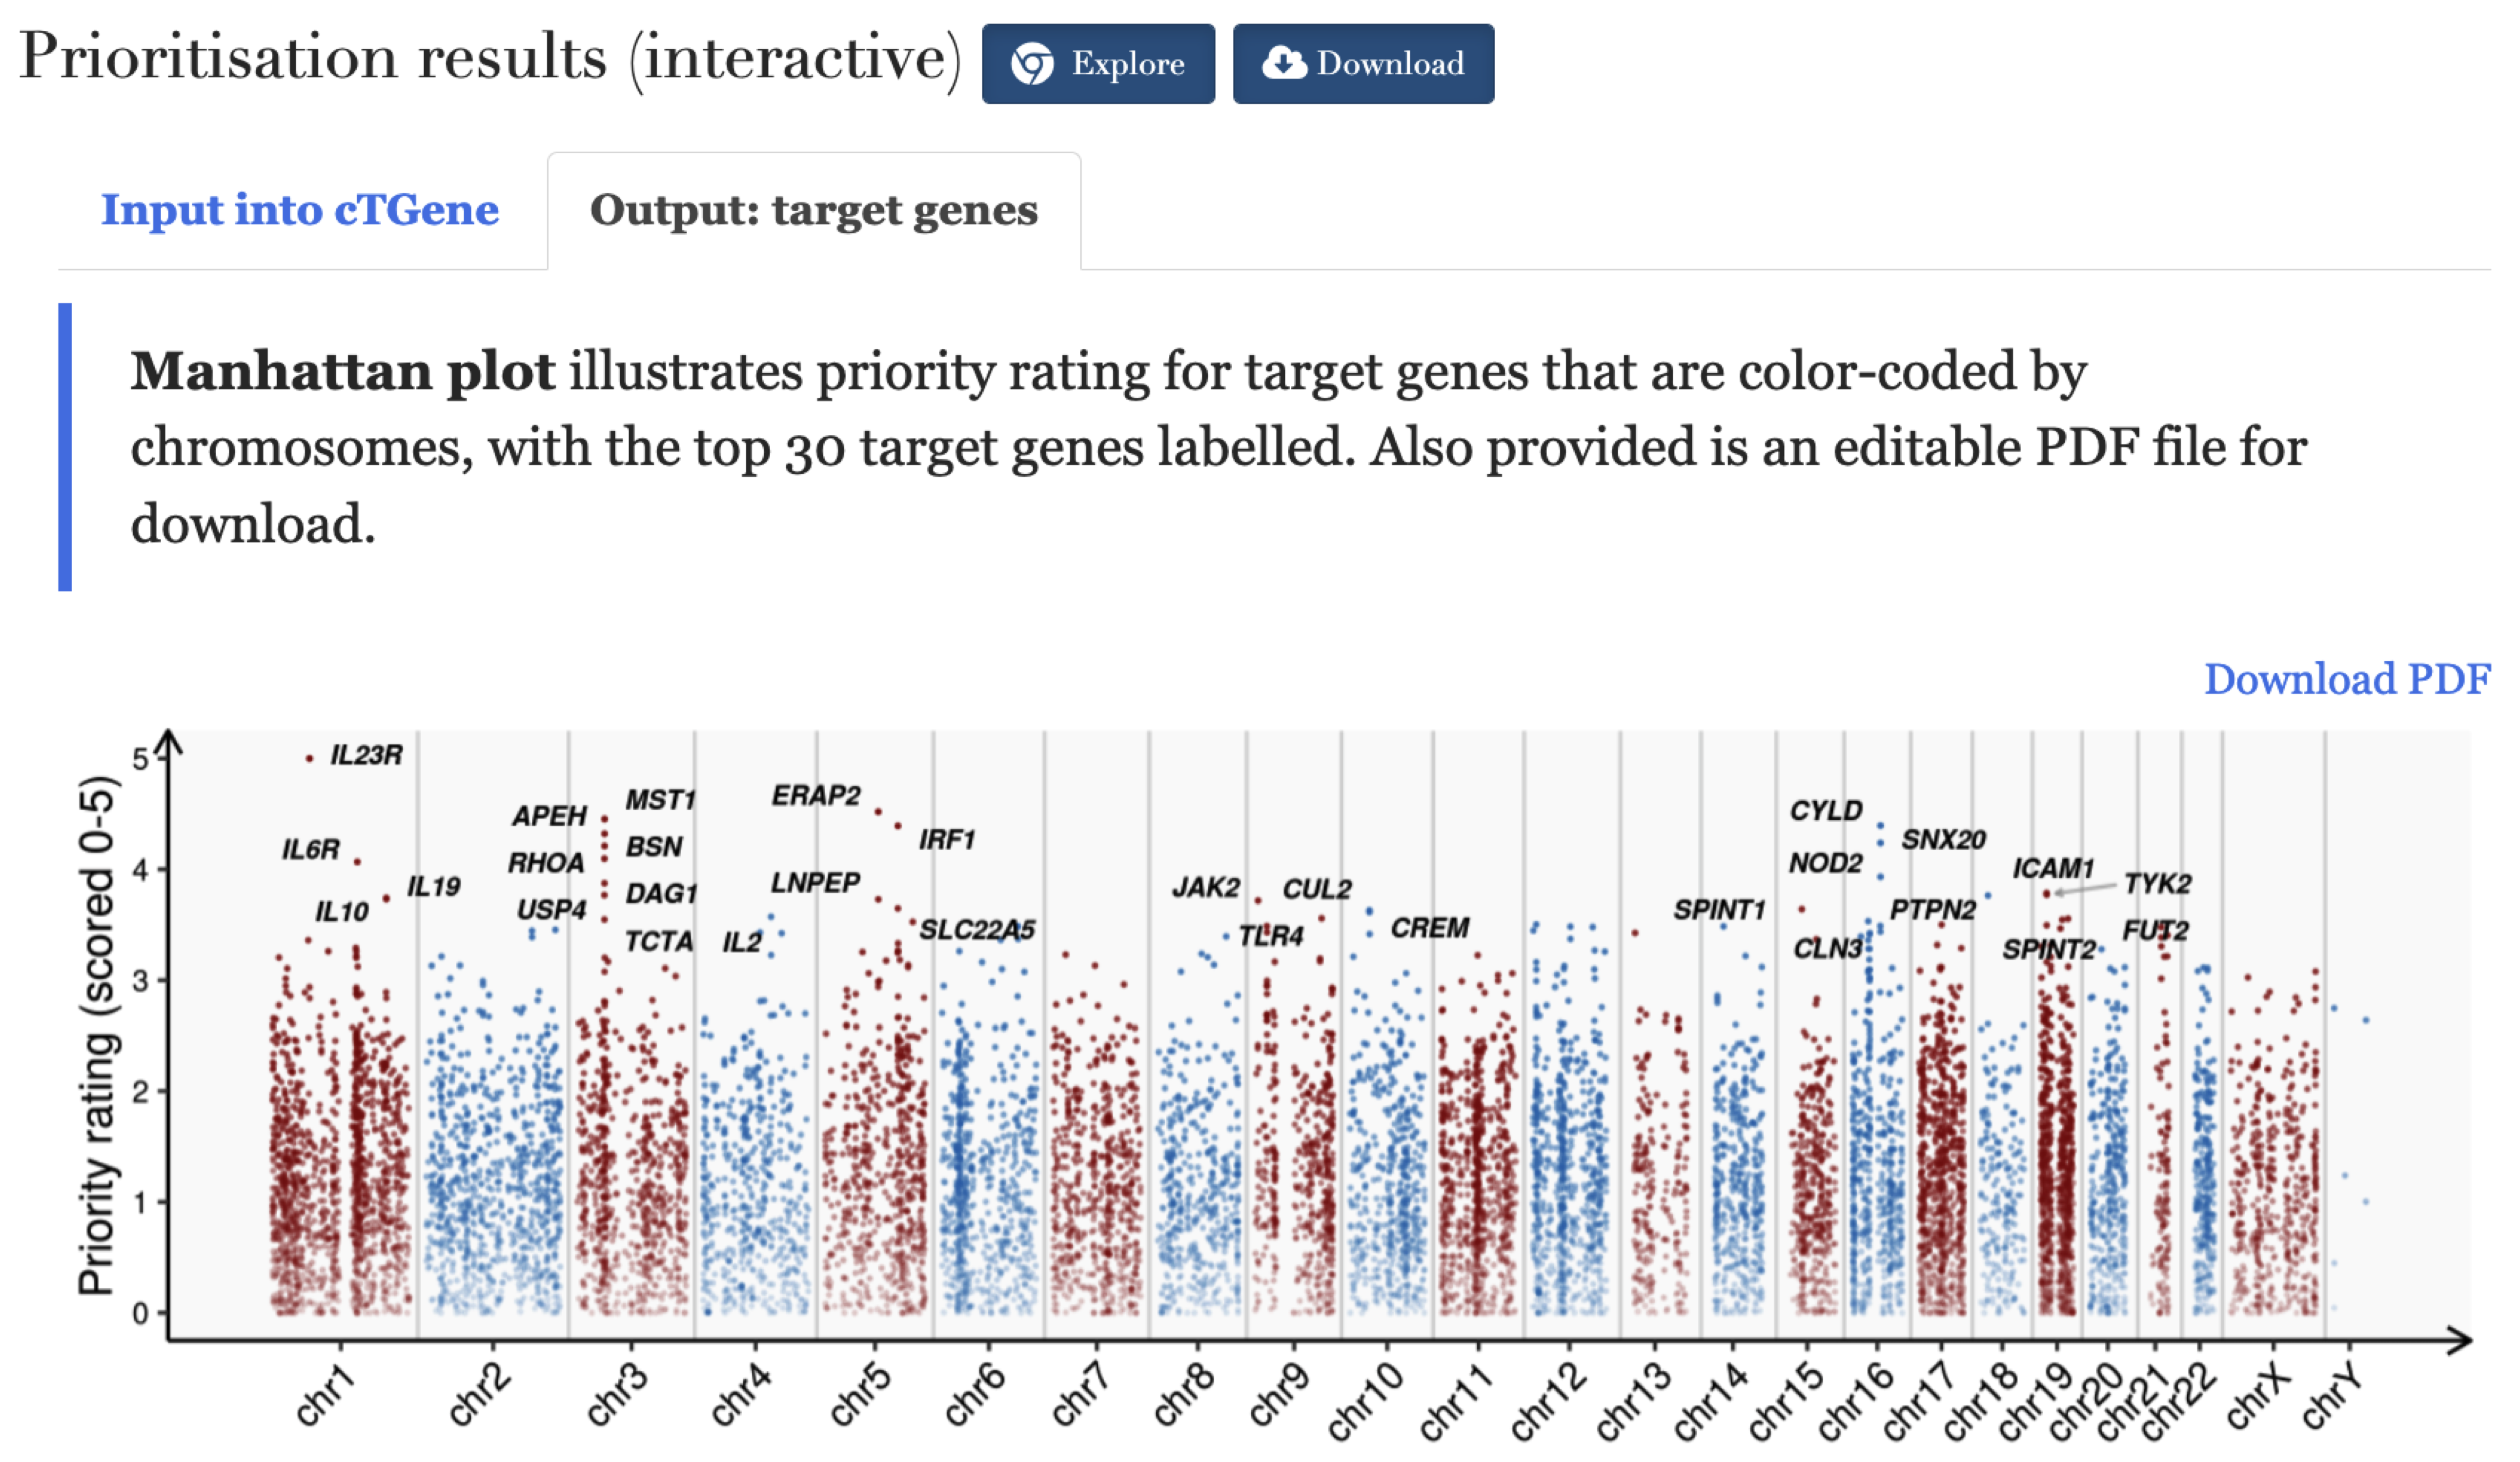
\includegraphics[width=0.8\linewidth]{index_files/figure-latex/cTGene-results-1} 

}

\caption{Prioritisation results for the `cTGene`. Under the tab `Output: target genes` is a manhattan plot illustrating priority rating for target genes. The user-input data under the tab `Input into cTGene` are also returned for the exploration.}\label{fig:cTGene-results}
\end{figure}

\begin{figure}

{\centering 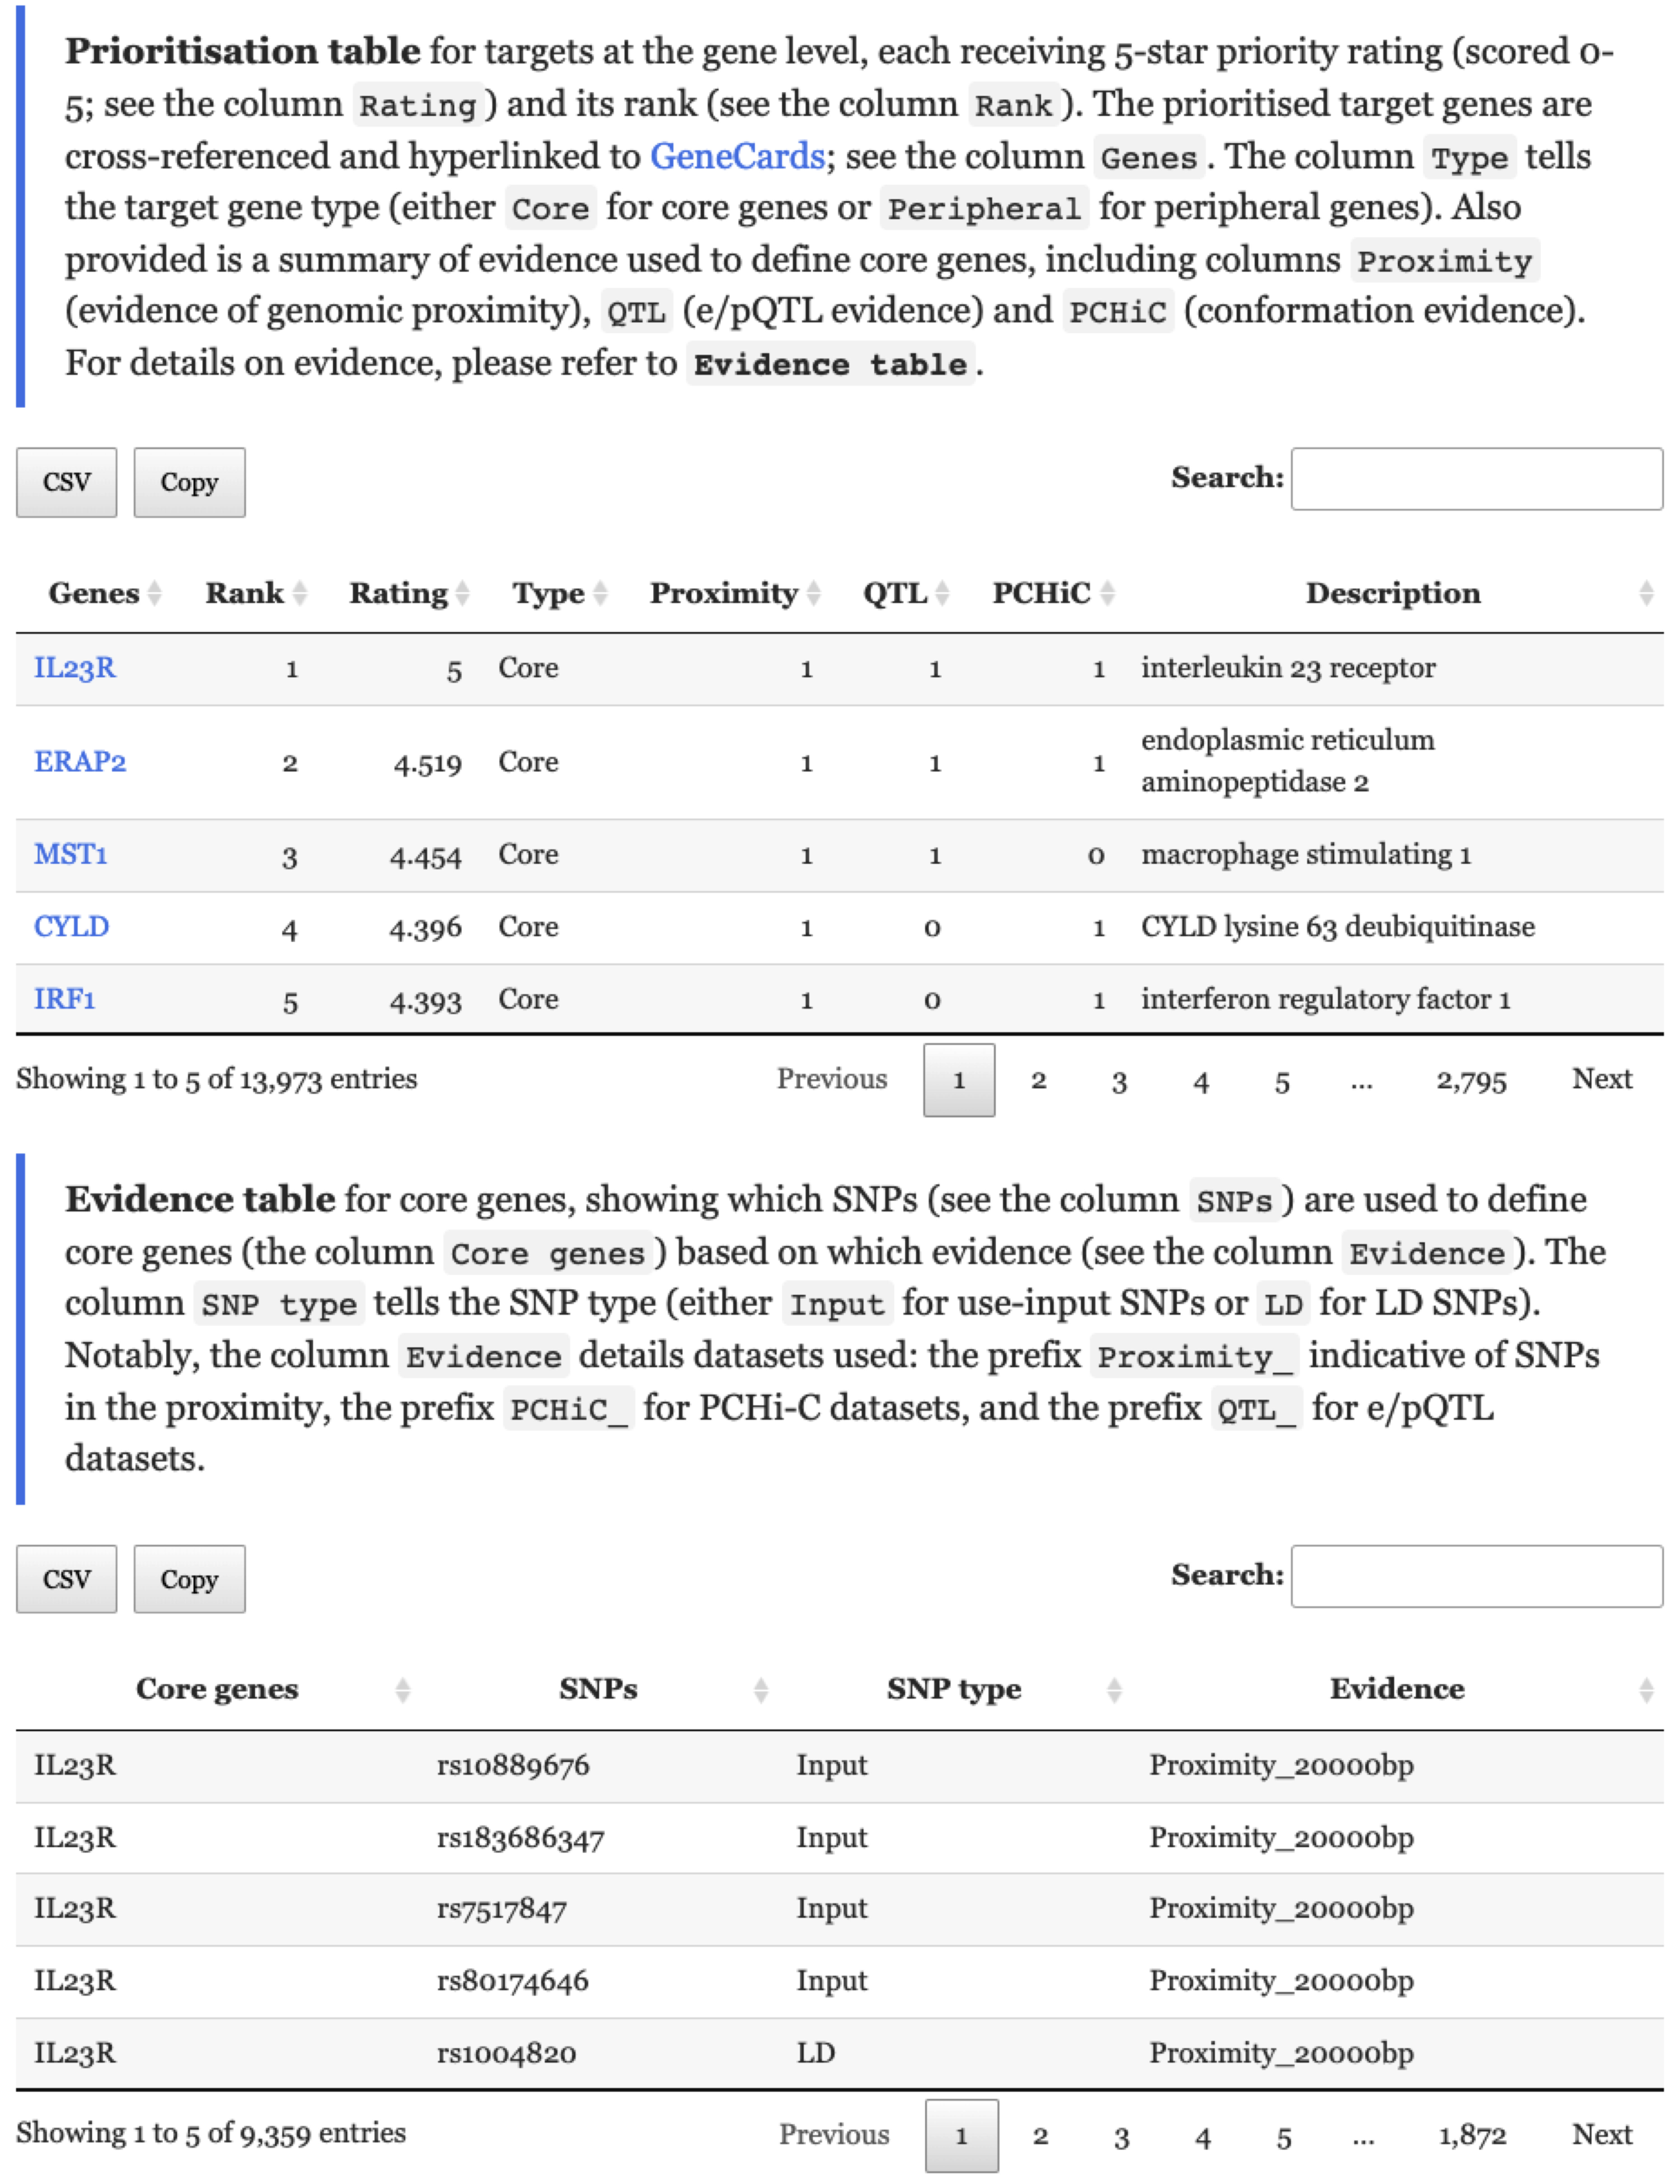
\includegraphics[width=0.9\linewidth]{index_files/figure-latex/cTGene-evidence-1} 

}

\caption{Two tabular displays about target genes (top) and evidence (bottom) under the tab `Output: target genes`.}\label{fig:cTGene-evidence}
\end{figure}

\hypertarget{ctcrosstalk}{%
\chapter{cTCrosstalk}\label{ctcrosstalk}}

\hypertarget{interface-4}{%
\section{Interface}\label{interface-4}}

\begin{quote}
\textbf{Input}
\end{quote}

\begin{itemize}
\tightlist
\item
  \texttt{Step\ 1}: a list of user-input SNPs, with 1st column for dbSNP rsIDs and 2nd column for significance info (p-values between 0 and 1). The error message will be displayed if the input is invalid. Example input data are shared genetic variants identified from cross-disease genome-wide association studies in inflammatory disorders; see \href{https://www.ncbi.nlm.nih.gov/pubmed/26974007}{Nature Genetics 2016}.
\end{itemize}

\begin{quote}
\textbf{Mechanism}
\end{quote}

\begin{itemize}
\item
  \texttt{Step\ 2}: includes SNPs in Linkage Disequilibrium (LD). By default, input SNPs with a typical threshold (p-value \textless{} 5e−8) are considered, and additional SNPs in linkage disequilibrium (R2 \textless{} 0.8) can be also included according to the European population.
\item
  \texttt{Step\ 3}: uses functional genomic datasets, including genomic proximity, quantitative trait locus (QTL) and promoter capture Hi-C (PCHi-C), to identify core genes.
\item
  \texttt{Step\ 4}: networks core genes with each other and with additional (peripheral) genes based on the knowledge of protein interactions, generating a ranked list of core and peripheral genes. It is achieved using the random walk with restart (RWW) algorithm. By default, the restarting probability of 0.7 is set, empirically optimised for immune-mediated diseases; selecting a value smaller than 0.6 is not recommended as there is a higher chance to expect low performance.
\item
  \texttt{Step\ 5}: identifies the subnetwork of highly-ranked genes that mediate the crosstalk between molecular pathways. The significance (p-value) of observing the identified crosstalk by chance is estimated by a degree-preserving node permutation test.
\item
  \texttt{More\ Controls}: fine-tunes parameters involved in steps described above.
\end{itemize}

\begin{quote}
\textbf{Output}
\end{quote}

\begin{itemize}
\tightlist
\item
  \href{/app/examples/_tmp_RMD_cTCrosstalk.html}{Example Output} includes target genes, target pathways, targets at the crosstalk level, and crosstalk-based drug repurposing. A summary of input data and the runtime (computed on the server side) is also returned to the users for the reference.
\end{itemize}

\begin{figure}

{\centering \includegraphics[width=1\linewidth]{index_files/figure-latex/cTCrosstalk-interface-1} 

}

\caption{The interface of the `cTCrosstalk`, enabling/automating genetics-led and network-based identification and prioritisation of drug targets at the crosstalk level. The `Show/Hide Info` toggle button contains the help information on how to use the `cTCrosstalk`, including input, output, mechanism, etc.}\label{fig:cTCrosstalk-interface}
\end{figure}

\hypertarget{prioritisation-results-1}{%
\section{Prioritisation results}\label{prioritisation-results-1}}

\begin{itemize}
\item
  \texttt{Output:\ target\ genes}: includes \texttt{Manhattan\ plot} illustrating priority rating for target genes that are color-coded by chromosomes. Also provided is the downloadable PDF file. It also includes \texttt{Prioritisation\ table} listing all prioritised genes, each receiving 5-star priority rating (scored 0-5), and \texttt{Evidence\ table} for core genes showing which SNPs are used to define core genes based on which evidence. Genes are cross-referenced and hyperlinked to GeneCards.
\item
  \texttt{Output:\ target\ pathways}: includes a dot plot and a prioritisation table for target pathways. Also provided is the downloadable PDF file.
\item
  \texttt{Output:\ targets\ at\ the\ crosstalk\ level}: includes \texttt{A\ network\ visualisation} illustrating the crosstalk between pathways, with genes colored by priority rating and labelled in the form of \texttt{rating®rank}, \texttt{Prioritisation\ table}
  listing crosstalk genes, each receiving 5-star priority rating (scored 0-5), and \texttt{Evidence\ table} for pathway crosstalk genes, showing which SNPs are used to crosstalk genes based on which evidence. Genes are cross-referenced and hyperlinked to GeneCards.
\item
  \texttt{Output:\ crosstalk-based\ drug\ repurposing}: includes \texttt{A\ heatmap-like\ illustration} showing drug repurposing analysis of approved drugs (licensed medications) based on pathway crosstalk genes, with crosstalk genes on y-axis, disease indications on x-axis, red dots indexed in number and referenced beneath in the table where the information on approved drugs and mechanisms of action is detailed. It also includes \texttt{An\ interactive\ table} of crosstalk genes (the column \texttt{Crosstalk\ genes}), disease indications (the column \texttt{Disease\ indications}), approved drugs and mechanisms (the column \texttt{Approved\ drugs\ {[}mechanisms\ of\ action{]}}), and drug index (the column \texttt{Index}) shown above within the dot plot.
\end{itemize}

\begin{figure}

{\centering 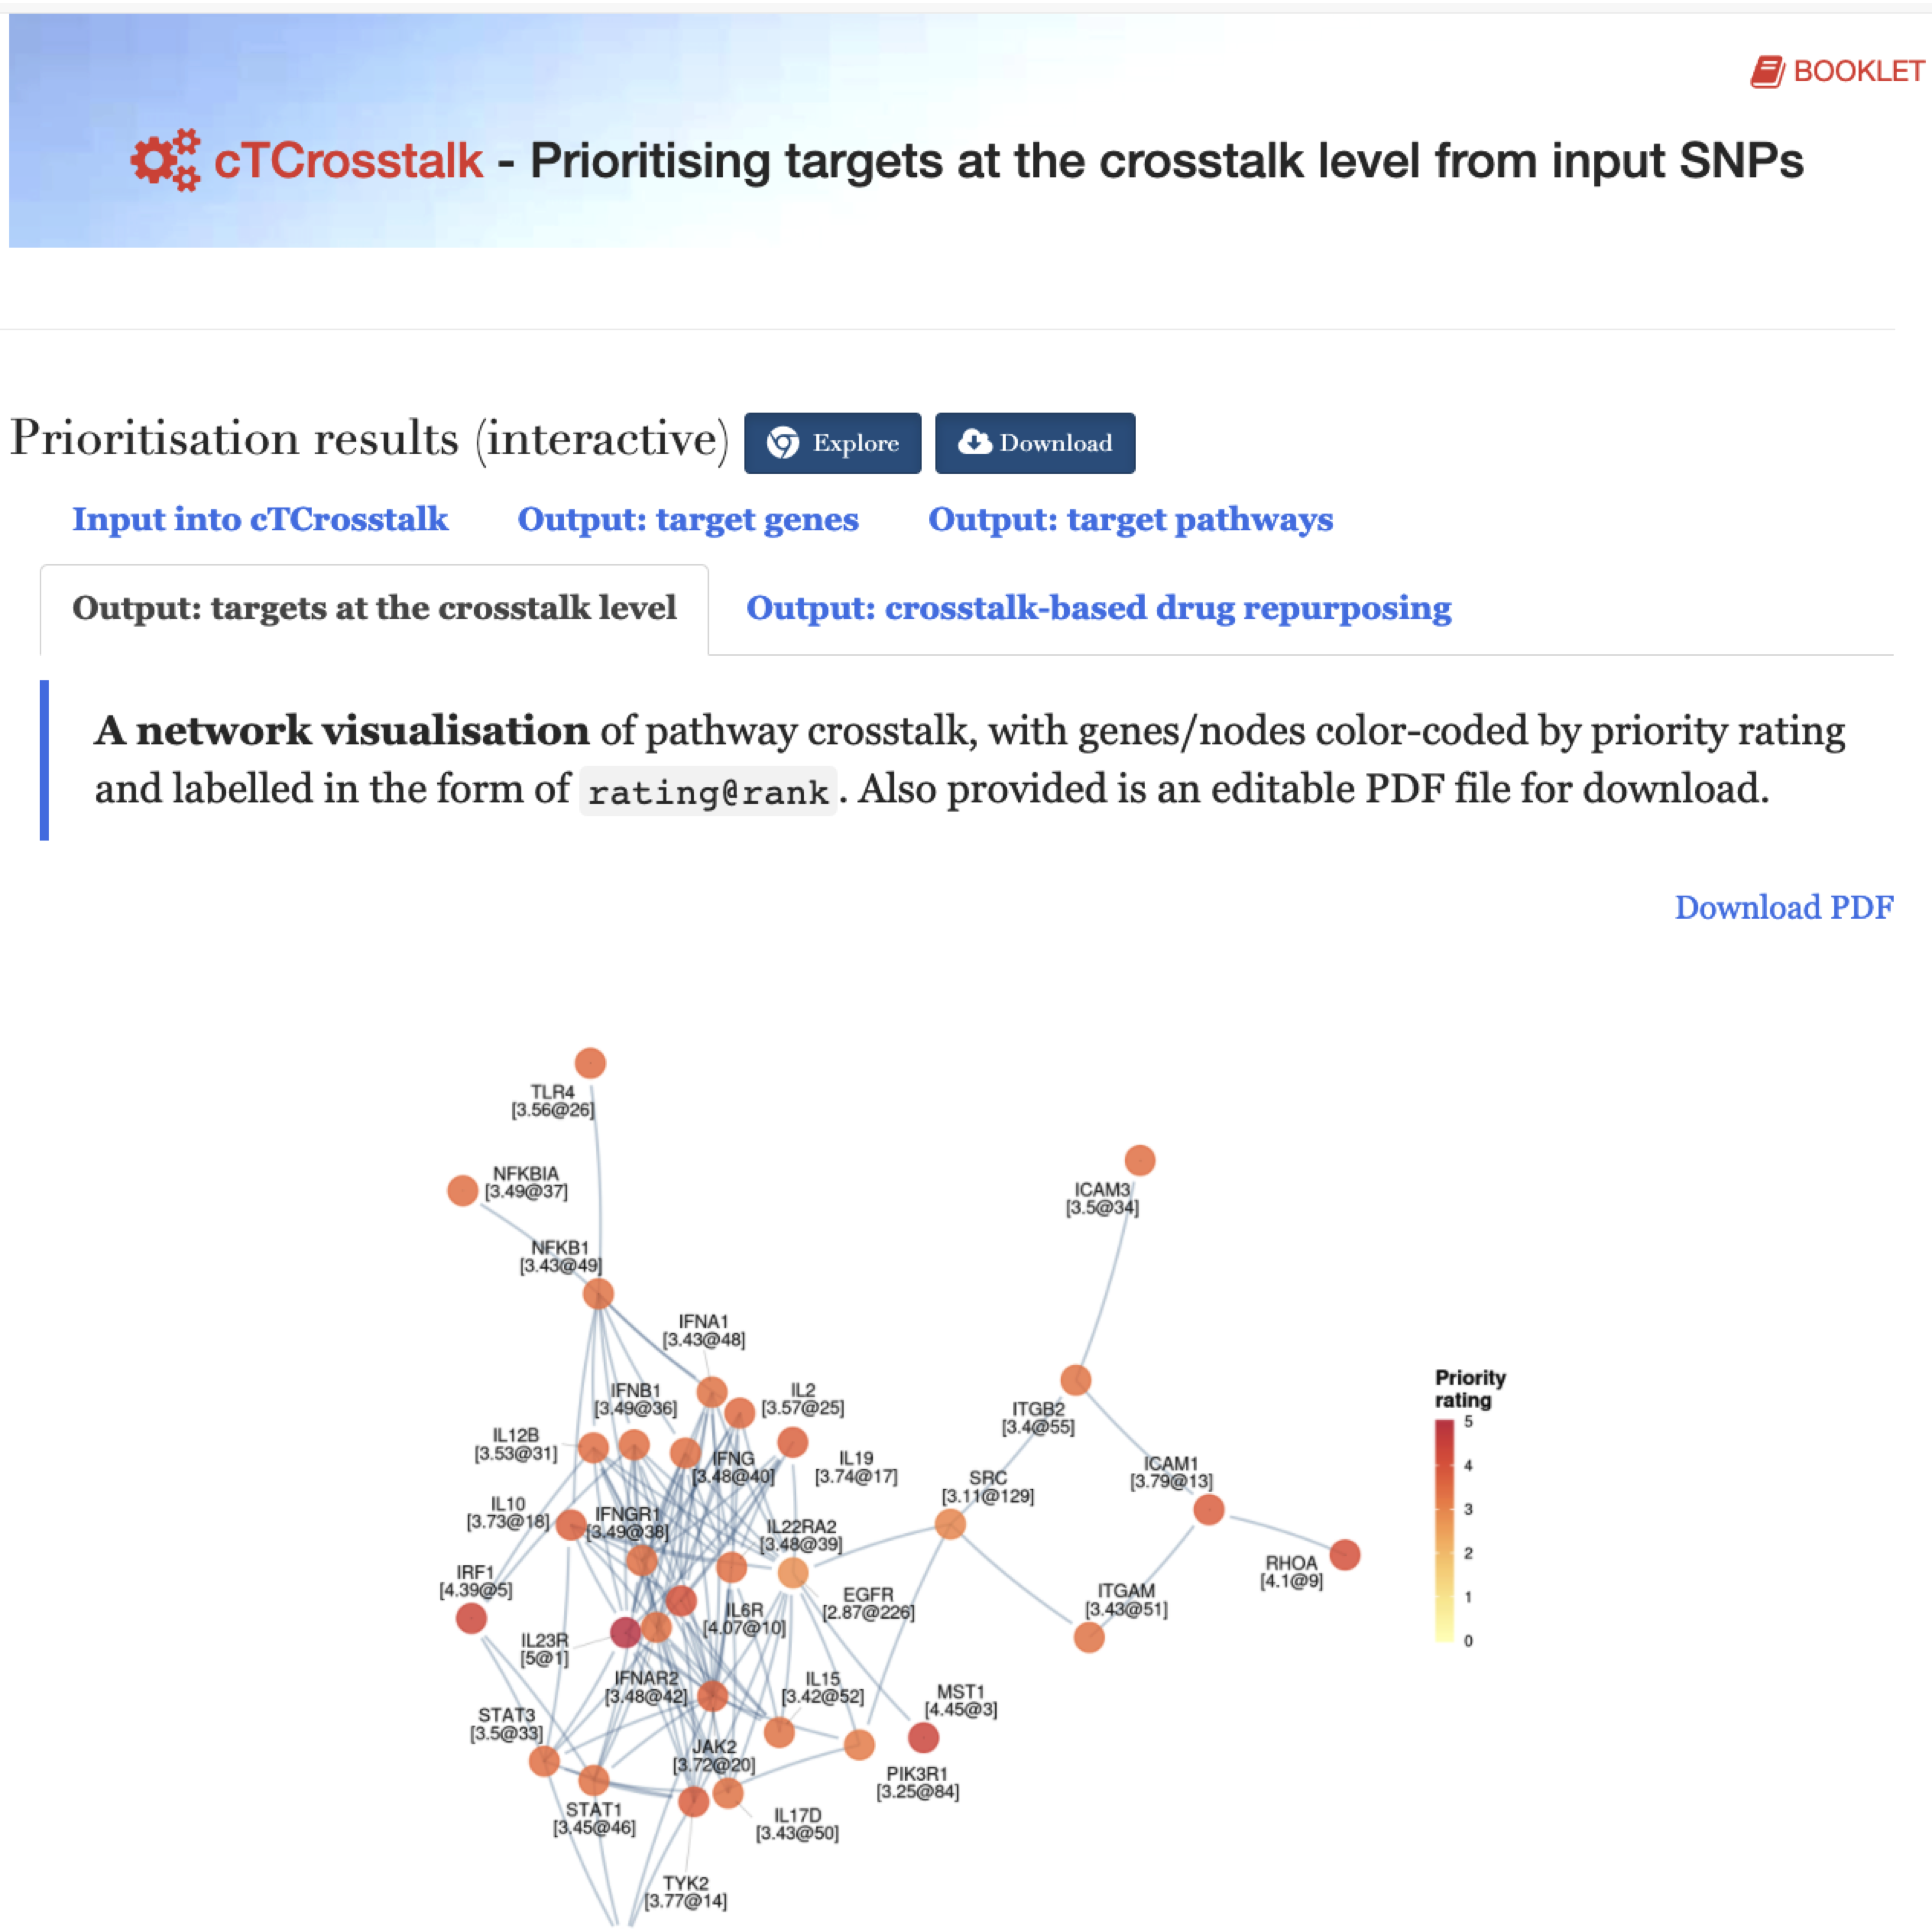
\includegraphics[width=0.8\linewidth]{index_files/figure-latex/cTCrosstalk-results-1} 

}

\caption{Prioritisation results for the `cTCrosstalk`. In addition to a summary of input data and the runtime (computed on the server side) under the tab `Input into cTCrosstalk`, the prioritisation results page provides the output, including target genes under the tab `Output: target genes` (the same as shown in the `cTGene`), target pathways under the tab `Output: target pathways`, and targets at the crosstalk level under the tab `Output: targets at the crosstalk level`, and crosstalk-based drug repurposing under the tab `Output: crosstalk-based drug repurposing`. Under the tab `Output: target genes` include  network visualisation of the crosstalk, with genes/nodes colour-coded by priority rating and labelled in the form of `rating®rank`, and two tabular displays about prioritisation and evidence for crosstalk genes.}\label{fig:cTCrosstalk-results}
\end{figure}

\begin{figure}

{\centering \includegraphics[width=0.8\linewidth]{index_files/figure-latex/cTCrosstalk-pathways-1} 

}

\caption{A dot plot for prioritised target pathways, with the top five labelled, available under the tab `Output: target pathways`. Also available is `Prioritisation table` for target pathways.}\label{fig:cTCrosstalk-pathways}
\end{figure}

\begin{figure}

{\centering 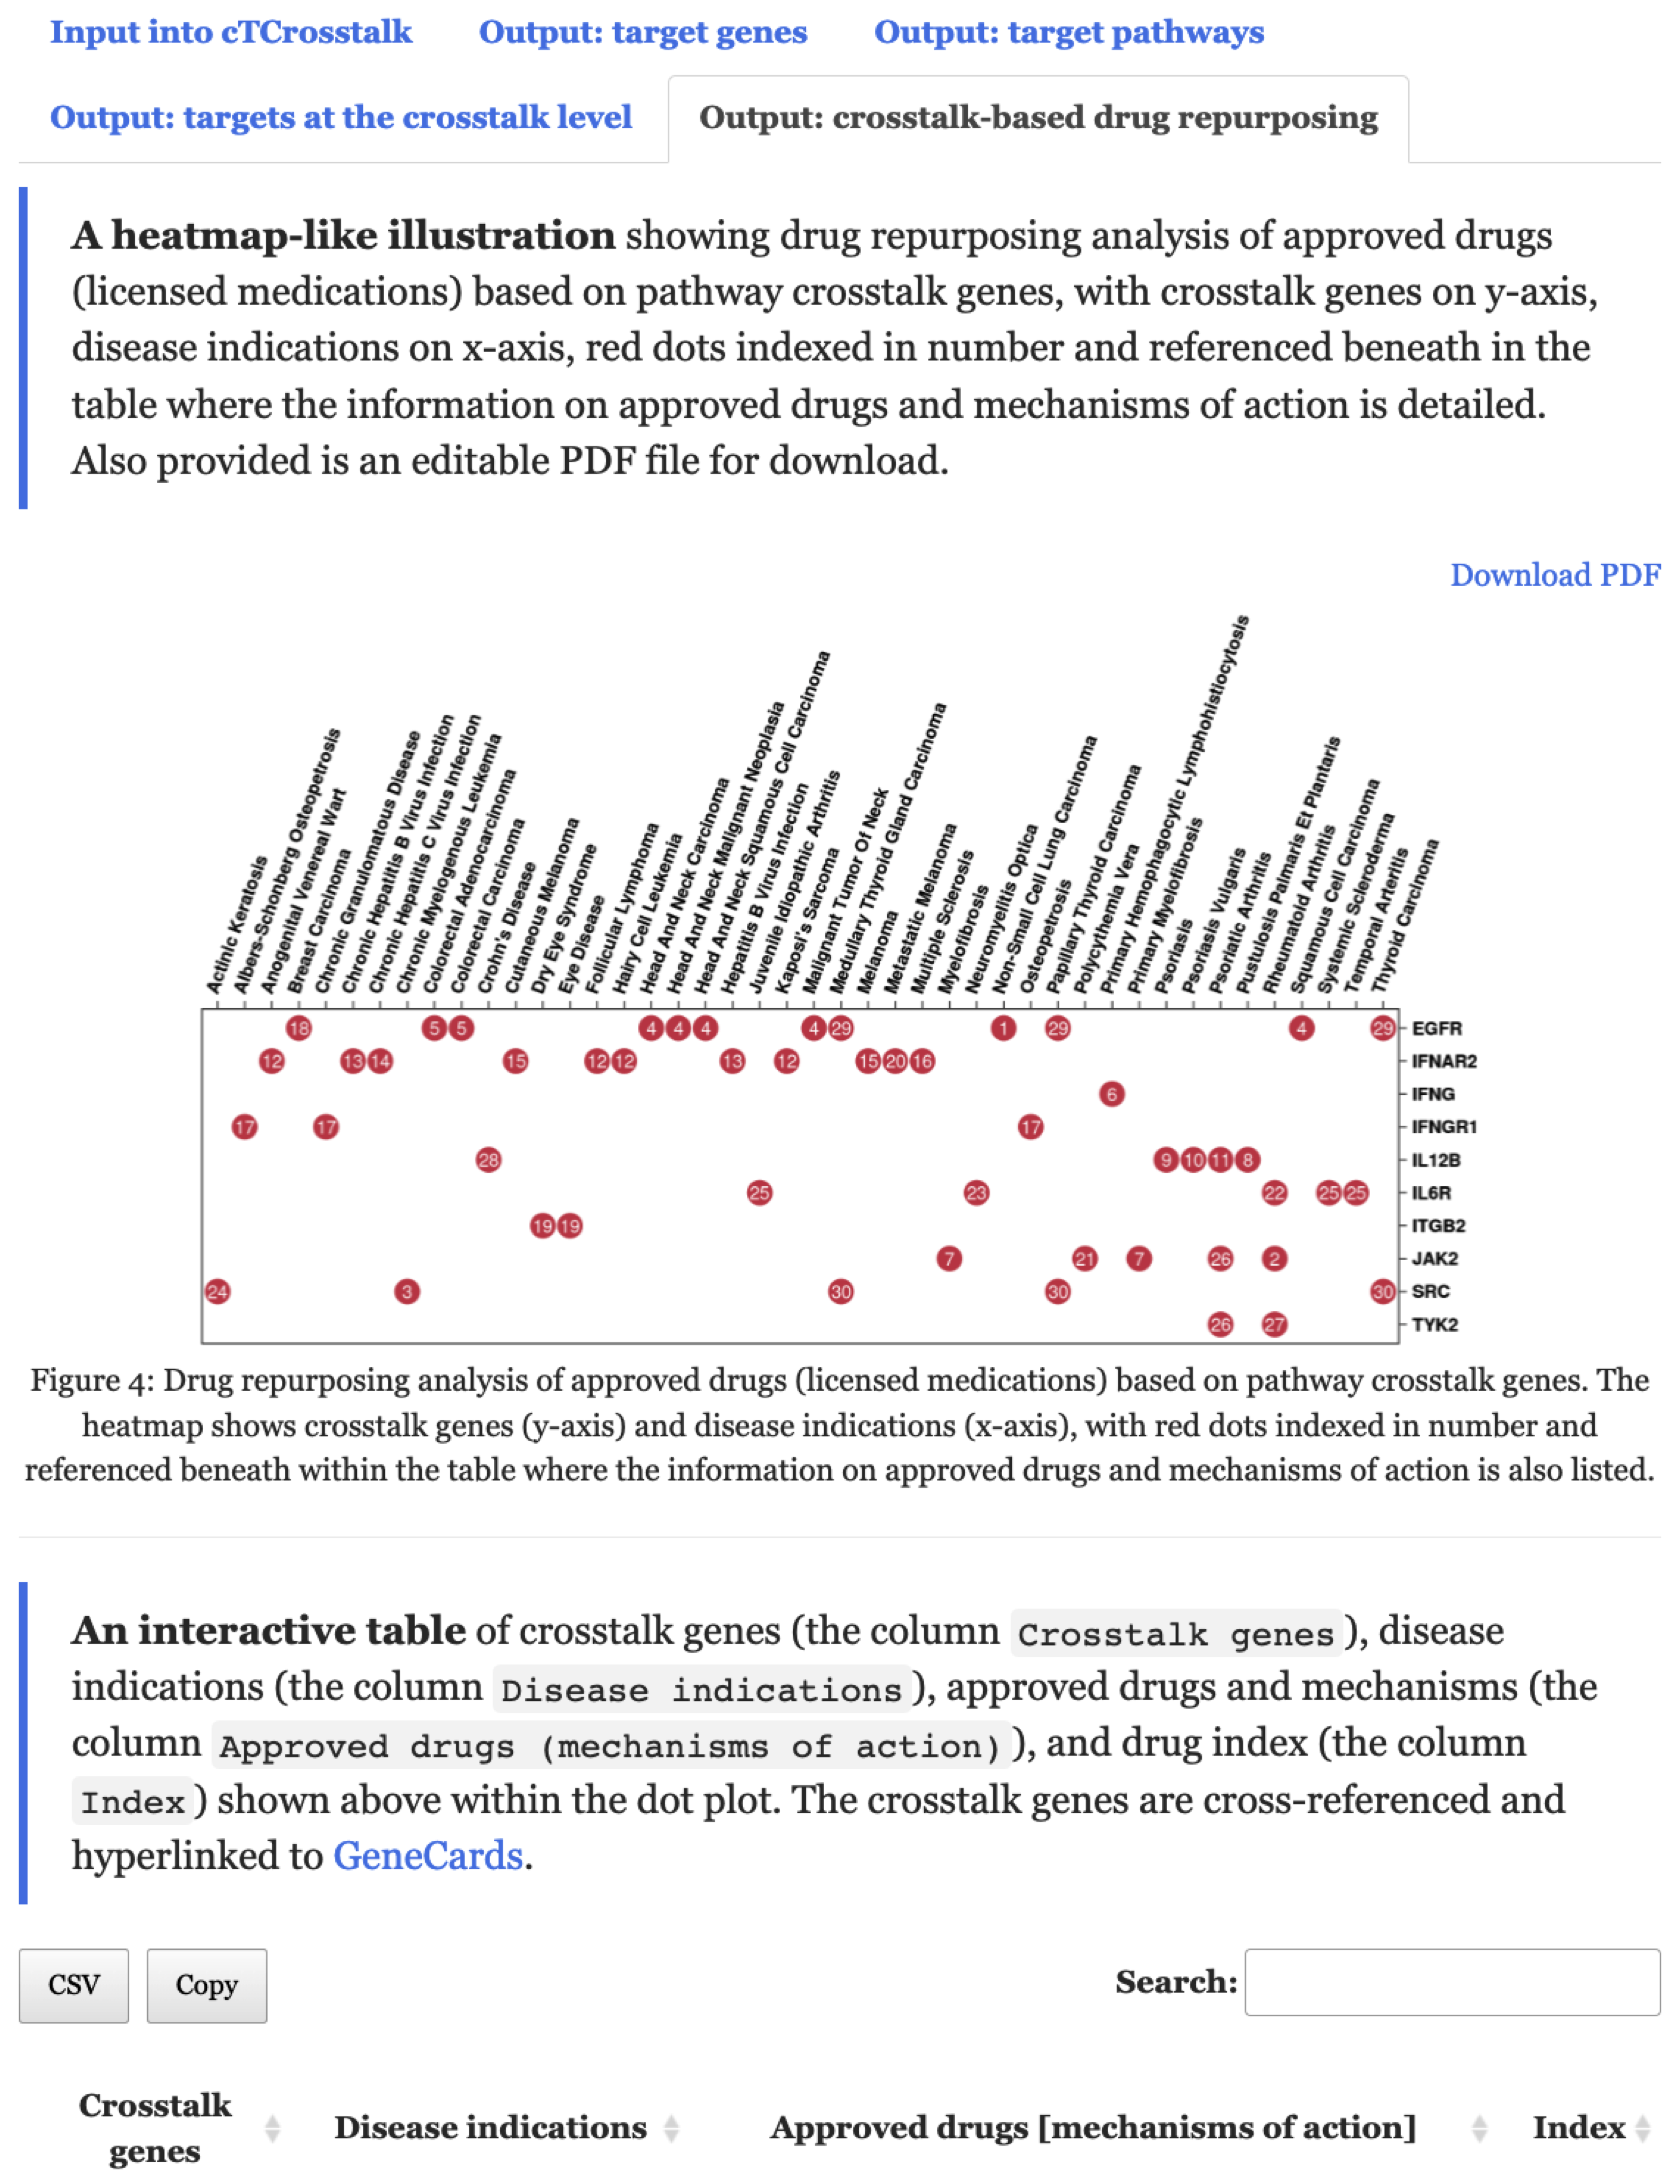
\includegraphics[width=0.9\linewidth]{index_files/figure-latex/cTCrosstalk-repurposing-1} 

}

\caption{A heatmap-like illustration, with crosstalk genes on the y-axis, disease indications on the x-axis, and red dots indexed in numbers under the tab `Output: crosstalk-based drug repurposing`. The index numbers are referenced in a table where the information on approved drugs and mechanisms of action is detailed.}\label{fig:cTCrosstalk-repurposing}
\end{figure}

\end{document}
